% =====================================================================
%  Decision Models  --  a lecture on "System One" models such as
%  TypeSafe's Jev: typed answers (choice, score, noul, box) with
%  calibrated probabilities instead of generated text; the primitives,
%  calibration and proper scoring rules, training (RLCD), selective
%  prediction and cascades, the landscape of decision models, their
%  limits, and how to use one inside an agent.
%  Same visual language as "The Transformer, Visually".
%
%  Compile:  pdflatex decision_models_tutorial.tex   (run twice)
%  Self-contained: every figure is TikZ/pgfplots source in this file.
%
%  Conventions
%   * \stage{n} before a frame sets the accent color and highlights the
%     matching chip in the footer strip.
%   * Numbers quoted from a paper or vendor documentation name the
%     source; numbers labelled "derived" were computed from quoted ones;
%     curves labelled "illustrative" are sketches, not data; $^\dagger$
%     marks vendor documentation, blogs and commentary.
% =====================================================================
\documentclass[aspectratio=169,11pt]{beamer}

% ---------- fonts ----------------------------------------------------
\usepackage[scaled=0.92]{helvet}        % Helvetica-like sans for text
\renewcommand{\ttdefault}{cmtt}         % Computer Modern mono for tokens
\usefonttheme[onlymath]{serif}          % classic serif math
\usepackage{amsmath,amssymb,bm}
\usepackage{booktabs,array}
\usepackage{graphicx}


% ---------- graphics -------------------------------------------------
\usepackage{tikz}
\usepackage{pgfplots}
\pgfplotsset{compat=1.17}
\usetikzlibrary{arrows.meta,positioning,calc,fit,backgrounds,
                decorations.pathreplacing,shapes.geometric}

% ---------- palette --------------------------------------------------
\definecolor{ink}{HTML}{1F2937}     % text, residual stream
\definecolor{muted}{HTML}{6B7280}   % secondary text
\definecolor{hair}{HTML}{D9DDE4}    % hairlines
\definecolor{paper}{HTML}{FCFCFA}   % slide background
\definecolor{tok}{HTML}{5F6F85}     % tokens / tokenizer
\definecolor{emb}{HTML}{0CA678}     % embeddings
\definecolor{posc}{HTML}{7048E8}     % positional information
\definecolor{attn}{HTML}{E8590C}    % attention
\definecolor{mlp}{HTML}{1C7ED6}     % MLP / feed-forward
\definecolor{norm}{HTML}{5C940D}    % normalization
\definecolor{outc}{HTML}{D6336C}     % unembedding / softmax / sampling
\definecolor{trn}{HTML}{9C6644}     % training and scaling
\colorlet{qc}{attn}                 % queries
\definecolor{kc}{HTML}{F59F00}      % keys
\definecolor{vc}{HTML}{1098AD}      % values
\colorlet{kct}{kc!70!black}         % key color, darkened for text
\colorlet{stagec}{ink}              % accent of the current stage

% ---------- beamer look ----------------------------------------------
\setbeamertemplate{navigation symbols}{}
\setbeamercolor{background canvas}{bg=paper}
\setbeamercolor{normal text}{fg=ink}
\setbeamercolor{frametitle}{fg=ink}
\setbeamersize{text margin left=8mm,text margin right=8mm}
\setbeamertemplate{itemize item}{\raisebox{0.25ex}{\tiny\color{stagec}$\blacksquare$}}
\setlength{\leftmargini}{1.1em}
\hyphenpenalty=10000 \exhyphenpenalty=10000   % no hyphenation on slides

% stage = which part of the pipeline the slide belongs to
\newcount\stageno \stageno=1
\newcommand{\stage}[1]{\global\stageno=#1\relax
  \ifcase#1\or\colorlet{stagec}{ink}\or\colorlet{stagec}{tok}%
  \or\colorlet{stagec}{emb}\or\colorlet{stagec}{attn}%
  \or\colorlet{stagec}{mlp}\or\colorlet{stagec}{posc}%
  \or\colorlet{stagec}{trn}\or\colorlet{stagec}{outc}%
  \or\colorlet{stagec}{vc}\or\colorlet{stagec}{ink}\fi}

\makeatletter
% title: accent bar + title + one-line claim (the frame subtitle)
\setbeamertemplate{frametitle}{%
  \nointerlineskip\vspace*{3.6mm}%
  \begin{tikzpicture}[x=1mm,y=1mm]
    \useasboundingbox (0,0) rectangle (144,10.5);
    \fill[stagec,rounded corners=0.5mm] (0,0.3) rectangle (1.5,10.2);
    \ifx\insertframesubtitle\@empty
      \node[anchor=west,inner sep=0,text=ink,
            font=\fontsize{15}{17}\selectfont\bfseries] at (4.2,5.2) {\insertframetitle};
    \else
      \node[anchor=west,inner sep=0,text=ink,
            font=\fontsize{15}{17}\selectfont\bfseries] at (4.2,7.1) {\insertframetitle};
      \node[anchor=west,inner sep=0,text=muted,
            font=\fontsize{8.6}{10}\selectfont] at (4.2,2.0) {\insertframesubtitle};
    \fi
  \end{tikzpicture}}
\makeatother

% footer: pipeline strip with the current stage lit, plus page number
\setbeamertemplate{footline}{%
  
\begin{tikzpicture}[x=1mm,y=1mm]
    \useasboundingbox (0,0) rectangle (160,7.2);
    \coordinate (c0) at (7.2,4.0);
    \foreach \lab/\col [count=\i,remember=\i as \prev (initially 0)] in
      {Overview/ink,Primitives/tok,Calibration/emb,Training/attn,Selection/mlp,
       Landscape/posc,Limits/trn,Evaluation/outc,Practice/vc,Wrap-up/ink}{
      \ifnum\i=\stageno
        \node[anchor=west,inner xsep=1.5mm,inner ysep=0.75mm,rounded corners=0.7mm,
              fill=\col,text=white,text height=1.5ex,text depth=0.35ex,
              font=\fontsize{5.8}{7}\selectfont\bfseries] (c\i) at ([xshift=0.8mm]c\prev.east) {\lab};
      \else
        \node[anchor=west,inner xsep=1.5mm,inner ysep=0.75mm,
              text=muted!80,text height=1.5ex,text depth=0.35ex,
              font=\fontsize{5.8}{7}\selectfont] (c\i) at ([xshift=0.8mm]c\prev.east) {\lab};
      \fi}
    \node[anchor=east,inner sep=0,text=muted,
          font=\fontsize{6.5}{8}\selectfont] at (152,4.0)
          {\insertframenumber\,/\,\inserttotalframenumber};
  \end{tikzpicture}}

% ---------- TikZ vocabulary ------------------------------------------
\tikzset{
  >={Stealth[length=4.6pt,width=4pt]},
  flow/.style={->,line width=0.8pt,draw=ink!70},
  thinflow/.style={->,line width=0.5pt,draw=ink!55},
  % component box (tinted) and its solid variant; argument = color
  comp/.style={rounded corners=2.2pt,draw=#1,fill=#1!12,line width=0.8pt,
               align=center,inner sep=4pt,font=\small,text=ink},
  fillbox/.style={rounded corners=2.2pt,fill=#1,text=white,align=center,
                inner sep=4pt,font=\small\bfseries},
  % a token
  chip/.style={rounded corners=1.8pt,fill=tok!14,draw=tok!55,line width=0.5pt,
               font=\ttfamily\footnotesize,inner xsep=3.5pt,inner ysep=2.5pt,
               text height=1.5ex,text depth=0.45ex,text=ink},
  cchip/.style={chip,fill=#1!16,draw=#1!75},
  lab/.style={font=\scriptsize,text=muted,inner sep=1.5pt},
  txt/.style={font=\footnotesize,text=ink,align=flush left,inner sep=0pt},
  plus/.style={circle,draw=ink,fill=paper,line width=0.75pt,inner sep=0pt,
               minimum size=9.5pt,font=\scriptsize\bfseries},
  brace/.style={decorate,decoration={brace,amplitude=3.5pt},draw=muted,line width=0.6pt},
}

% \cells{x}{y}{size}{color}{shade,shade,...}: a row of vector cells
\newcommand{\cells}[5]{%
  \foreach \sh [count=\ci from 0] in {#5}{%
    \fill[#4!\sh!white,draw=paper,line width=0.4pt]
      ({#1+\ci*#3},{#2}) rectangle ++(#3,#3);}}

% \rgrid{x}{y}{rows}{cols}{size}{color}{seed}: a matrix with varied shading
\newcommand{\rgrid}[7]{%
  \foreach \ri in {1,...,#3}{\foreach \ci in {1,...,#4}{%
    \pgfmathtruncatemacro\sh{16+mod(\ri*37+\ci*53+\ri*\ci*11+#7*29,8)*10}%
    \fill[#6!\sh!white,draw=paper,line width=0.4pt]
      ({#1+(\ci-1)*#5},{#2+(#3-\ri)*#5}) rectangle ++(#5,#5);}}}

% \barh{x}{y}{length}{color}: one horizontal bar of a bar chart
\newcommand{\barh}[4]{\fill[#4,rounded corners=0.8pt] ({#1},{#2-0.13}) rectangle ++({#3},0.26);}

% \valgrid{x}{y}{size}{color}{scale}{mask}{\rows}: matrix shaded by value.
% (x,y) is the top-left corner; \rows is a macro holding {a,b,..},{..},..
% With mask=1 the cells above the diagonal are drawn as blocked.
\newcommand{\valgrid}[7]{%
  \edef\vglist{#7}%
  \foreach \row [count=\r from 0] in \vglist {\foreach \v [count=\c from 0] in \row {%
    \pgfmathtruncatemacro\sh{min(100,\v*#5)}%
    \pgfmathtruncatemacro\msk{and(#6>0,\c>\r)}%
    \ifnum\msk=1
      \fill[tok!10,draw=paper,line width=0.4pt] ({#1+\c*#3},{#2-(\r+1)*#3}) rectangle ++(#3,#3);
    \else
      \fill[#4!\sh!white,draw=paper,line width=0.4pt] ({#1+\c*#3},{#2-(\r+1)*#3}) rectangle ++(#3,#3);
    \fi}}}

% the running attention example: Alice thanked Bob because she
\def\Sraw{{2.0,0.7,1.3,0.4,1.1},{1.8,1.2,0.9,1.6,0.5},{0.6,1.5,1.9,0.8,1.4},
          {0.8,1.6,0.9,1.1,2.1},{3.1,0.9,1.4,1.0,1.5}}          % scores
\def\Aw{{1.00,0,0,0,0},{.65,.35,0,0,0},{.14,.35,.51,0,0},
        {.18,.39,.19,.24,0},{.62,.07,.11,.08,.12}}              % softmax rows

% paper figure: \paperfig{file}{width}{Figure n}
\newcommand{\paperfig}[3]{%
  \begin{tikzpicture}
    \node[inner sep=0] (img) {\includegraphics[width=#2]{#1}};
    \node[anchor=north east,font=\fontsize{5.5}{6}\selectfont,text=muted,
          rounded corners=1pt,fill=ink!6,inner sep=2pt] at ([xshift=-1mm,yshift=-1mm]img.north east) {report, #3};
  \end{tikzpicture}}
% background panel: \bgpanel{x}{y}{width}{title}{body}  (anchor north west)
\newcommand{\bgpanel}[5]{%
  \node[anchor=north west,inner sep=0] at (#1,#2) {%
    \begin{tikzpicture}
      \node[anchor=north west,text width=#3,align=flush left,font=\footnotesize,text=ink,
            inner xsep=8pt,inner ysep=6pt,rounded corners=3pt,fill=stagec!7] (bp)
            {{\color{stagec}\bfseries\scriptsize #4}\\[3pt]#5};
      \fill[stagec,rounded corners=1.5pt] (bp.north west) rectangle ([xshift=3pt]bp.south west);
    \end{tikzpicture}};}
% same panel with a smaller body font, for denser slides
\newcommand{\bgpanels}[5]{%
  \node[anchor=north west,inner sep=0] at (#1,#2) {%
    \begin{tikzpicture}
      \node[anchor=north west,text width=#3,align=flush left,font=\scriptsize,text=ink,
            inner xsep=8pt,inner ysep=6pt,rounded corners=3pt,fill=stagec!7] (bp)
            {{\color{stagec}\bfseries\scriptsize #4}\\[3pt]#5};
      \fill[stagec,rounded corners=1.5pt] (bp.north west) rectangle ([xshift=3pt]bp.south west);
    \end{tikzpicture}};}
% stat tile: \stat{x}{y}{value}{label}{color}
\newcommand{\stat}[5]{%
  \node[anchor=north west,inner sep=0] at (#1,#2) {%
    \begin{tikzpicture}
      \node[anchor=north west,minimum width=3.2cm,minimum height=1.45cm,rounded corners=3pt,
            fill=#5!10,draw=#5!50,line width=0.6pt] (t) {};
      \node[anchor=north west,font=\fontsize{15}{16}\selectfont\bfseries,text=#5!85!black,inner sep=0]
            at ([xshift=7pt,yshift=-7pt]t.north west) {#3};
      \node[anchor=south west,font=\scriptsize,text=ink,inner sep=0,text width=2.9cm,align=left]
            at ([xshift=7pt,yshift=6pt]t.south west) {#4};
    \end{tikzpicture}};}

% small source tag inside a figure: \srctag{x}{y}{text}
\newcommand{\srctag}[3]{\node[anchor=north east,font=\fontsize{5.5}{6}\selectfont,text=muted,
  rounded corners=1pt,fill=ink!6,inner sep=2pt] at (#1,#2) {#3};}
% axis style shared by all plots
\pgfplotsset{lecture/.style={axis lines=left,axis line style={muted,line width=0.5pt},
  tick style={muted},tick label style={font=\scriptsize,text=muted},
  label style={font=\scriptsize,text=muted},grid=major,grid style={hair,line width=0.4pt},
  legend style={draw=none,fill=none,font=\scriptsize,legend cell align=left,row sep=1pt},
  clip=false}}

% chat message: \msg{x}{y}{width}{role color}{role}{text}  (anchor north west)
\newcommand{\msg}[6]{%
  \node[anchor=north west,inner sep=0] at (#1,#2) {%
    \begin{tikzpicture}
      \node[anchor=north west,text width=#3,align=flush left,font=\scriptsize,text=ink,
            inner xsep=5pt,inner ysep=4pt,rounded corners=3pt,fill=#4!8,draw=#4!35,line width=0.4pt] (m) {#6};
      \node[anchor=south west,font=\tiny\bfseries,text=#4,inner sep=1pt] at ([yshift=0.5pt]m.north west) {#5};
    \end{tikzpicture}};}
% pipeline chevron: \chev{x}{y}{width}{color}{label}
\newcommand{\chev}[5]{%
  \fill[#4,rounded corners=1pt] (#1,#2) -- ({#1+#3-0.22},#2) -- ({#1+#3},{#2+0.3}) -- ({#1+#3-0.22},{#2+0.6}) -- (#1,{#2+0.6}) -- ({#1+0.22},{#2+0.3}) -- cycle;
  \node[text=white,font=\scriptsize\bfseries] at ({#1+#3/2},{#2+0.3}) {#5};}

% short text helpers
\newcommand{\hl}[2]{{\color{#1}\bfseries #2}}
\newcommand{\tokt}[1]{{\ttfamily #1}}
\begin{document}

% ---------------------------------------------------------------- 1
{\setbeamertemplate{footline}{}
\begin{frame}[plain]
\begin{tikzpicture}[remember picture,overlay,x=1mm,y=1mm,
                    shift={(current page.south west)}]
  % cover graphic: a question going in, a distribution coming out
  \begin{scope}[shift={(96,14)}]
    \node[anchor=south west,font=\fontsize{6.5}{7.5}\selectfont\ttfamily,text=ink,
          rounded corners=1.2mm,fill=ink!6,inner sep=2.5mm,text width=50mm,align=left] at (0,36)
      {state: "My card was charged twice."\\
       question: which team owns this?\\
       options: billing | bug | account | other};
    \draw[flow] (25,35) -- (25,30);
    \foreach \x/\h/\lab/\p in {0/26/billing/0.62,12/9/bug/0.21,24/5/account/0.12,36/2/other/0.05}{
      \fill[outc!80,rounded corners=0.8mm] (\x+2,0) rectangle (\x+10,\h);
      \node[font=\fontsize{5.5}{6}\selectfont,text=muted] at (\x+6,-3) {\lab};
      \node[font=\fontsize{5.5}{6}\selectfont\bfseries,text=outc!80!black] at (\x+6,\h+2.5) {\p};}
    \draw[muted,line width=0.5pt] (0,0) -- (48,0);
    \node[font=\fontsize{5.5}{6}\selectfont,text=muted,anchor=north east] at (48,-6) {confidence 0.49 (derived)};
  \end{scope}
  \fill[outc] (12,60.5) rectangle (26,61.6);
  \node[anchor=south west,inner sep=0,text=muted,
        font=\fontsize{10}{12}\selectfont\bfseries] at (12,63.5) {LECTURE NOTES \ $\cdot$ \ MODELS, 2026};
  \node[anchor=south west,inner sep=0,text=ink,align=left,
        font=\fontsize{30}{34}\selectfont\bfseries] at (12,38)
        {Decision\\Models};
  \node[anchor=north west,inner sep=0,text=muted,align=flush left,text width=78mm,
        font=\fontsize{10}{13}\selectfont] at (12,34)
        {Models that answer typed questions with calibrated probabilities
         instead of text: the primitives, calibration and how it is
         trained for, selective prediction and cascades, the 2026
         landscape around TypeSafe's Jev, the failure modes, and how to
         put one inside an agent.};
\end{tikzpicture}
\end{frame}}

% ---------------------------------------------------------------- 2
\stage{1}
\begin{frame}{A decision model answers typed questions with probabilities}
\framesubtitle{Same transformer lineage, different contract: a distribution over options you supplied, no text to parse.}
\centering
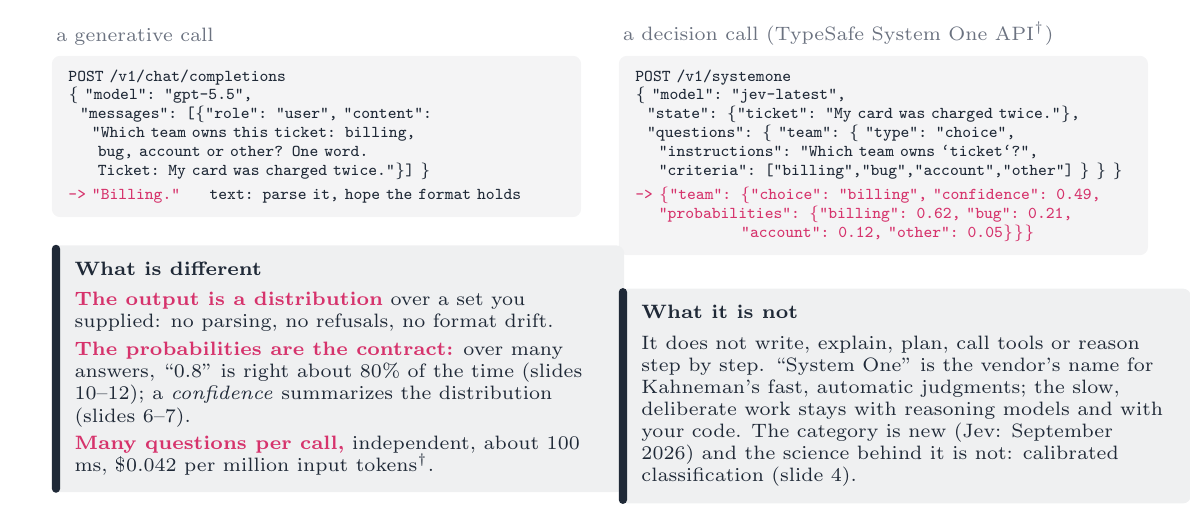
\begin{tikzpicture}
  \useasboundingbox (0,0) rectangle (14.4,5.9);
  \node[lab,anchor=south west] at (0.3,5.62) {a generative call};
  \node[anchor=north west,inner sep=0,font=\ttfamily\fontsize{5.8}{6.8}\selectfont,text=ink,
        rounded corners=3pt,fill=ink!5,inner xsep=6pt,inner ysep=5pt,text width=6.3cm,align=left] at (0.3,5.55) {%
    POST /v1/chat/completions\\
    \{ "model": "gpt-5.5",\\
    \ \ "messages": [\{"role": "user", "content":\\
    \ \ \ \ "Which team owns this ticket: billing,\\
    \ \ \ \ \ bug, account or other? One word.\\
    \ \ \ \ \ Ticket: My card was charged twice."\}] \}\\[2pt]
    {\color{outc}-> "Billing."} \ \ \ \ text: parse it, hope the format holds};
  \node[lab,anchor=south west] at (7.5,5.62) {a decision call (TypeSafe System One API$^\dagger$)};
  \node[anchor=north west,inner sep=0,font=\ttfamily\fontsize{5.8}{6.8}\selectfont,text=ink,
        rounded corners=3pt,fill=ink!5,inner xsep=6pt,inner ysep=5pt,text width=6.3cm,align=left] at (7.5,5.55) {%
    POST /v1/systemone\\
    \{ "model": "jev-latest",\\
    \ \ "state": \{"ticket": "My card was charged twice."\},\\
    \ \ "questions": \{ "team": \{ "type": "choice",\\
    \ \ \ \ "instructions": "Which team owns `ticket`?",\\
    \ \ \ \ "criteria": ["billing","bug","account","other"] \} \} \}\\[2pt]
    {\color{outc}-> \{"team": \{"choice": "billing", "confidence": 0.49,}\\
    {\color{outc}\ \ \ \ "probabilities": \{"billing": 0.62, "bug": 0.21,}\\
    {\color{outc}\ \ \ \ \ \ \ \ \ \ \ \ \ \ \ \ \ \ "account": 0.12, "other": 0.05\}\}\}}};
  \bgpanels{0.3}{3.15}{6.7cm}{What is different}{%
    \hl{outc}{The output is a distribution} over a set you supplied: no
    parsing, no refusals, no format drift.\\[2pt]
    \hl{outc}{The probabilities are the contract:} over many answers,
    ``0.8'' is right about 80\% of the time (slides 10--12); a
    \emph{confidence} summarizes the distribution (slides 6--7).\\[2pt]
    \hl{outc}{Many questions per call,} independent, about 100 ms,
    \$0.042 per million input tokens$^\dagger$.}
  \bgpanels{7.5}{2.6}{6.7cm}{What it is not}{%
    It does not write, explain, plan, call tools or reason step by step.
    ``System One'' is the vendor's name for Kahneman's fast, automatic
    judgments; the slow, deliberate work stays with reasoning models and
    with your code. The category is new (Jev: September 2026) and the
    science behind it is not: calibrated classification (slide 4).}
\end{tikzpicture}
\end{frame}

% ---------------------------------------------------------------- 3
\begin{frame}{Why now: an agent loop is full of small judgments}
\framesubtitle{Most of what an agent decides is a classification, a yes/no or a rating, and a generator is an expensive way to get one.}
\centering
\begin{tikzpicture}
  \useasboundingbox (0,0) rectangle (14.4,5.9);
  % the loop with decision badges
  \foreach \i/\x/\c/\ttl/\q in {
      0/0.3/tok/{request}/{},
      1/2.55/outc/{guard}/{noul: jailbreak? harmful?},
      2/4.8/outc/{route}/{choice: intent, tool, model},
      3/7.05/outc/{retrieve}/{score: passage relevance},
      4/9.3/mlp/{generate}/{reasoning model writes},
      5/11.55/outc/{verify}/{noul: cited? policy ok?}}{
    \node[anchor=north west,inner sep=0] at (\x,5.6) {%
      \begin{tikzpicture}
        \node[anchor=north west,minimum width=2.15cm,minimum height=0.62cm,rounded corners=3pt,fill=\c!10,draw=\c!55,line width=0.6pt] (b) {};
        \node[anchor=west,font=\scriptsize\bfseries,text=\c!85!black,inner sep=0] at ([xshift=6pt]b.west) {\ttl};
      \end{tikzpicture}};
    \node[lab,anchor=north west,text width=2.1cm,font=\tiny] at (\x,4.9) {\q};}
  \foreach \a/\b in {2.45/2.55,4.7/4.8,6.95/7.05,9.2/9.3,11.45/11.55}{\draw[flow] (\a,5.29) -- (\b,5.29);}
  \draw[flow,rounded corners=3pt] (13.7,5.0) -- (13.9,5.0) -- (13.9,4.2) -- (1.3,4.2) -- (1.3,4.95);
  \node[lab,anchor=north,font=\tiny] at (7.5,4.17) {act, or escalate to a person when confidence is low; then the next turn};
  \bgpanels{0.3}{3.6}{6.7cm}{Why a generator is the wrong tool for these}{%
    \hl{outc}{Cost and latency:} a frontier model lists \$5 per million
    input tokens and takes seconds; a decision model lists \$0.042 and
    answers in about 100 ms$^\dagger$: 120$\times$ cheaper per input token
    (derived), with no output tokens to pay for.\\[2pt]
    \hl{outc}{No probability:} asking a chat model ``how sure are you?''
    gives overconfident, clustered numbers (Xiong et al.\ 2023); its
    token logprobs drift after RLHF (GPT-4 report, 2023).\\[2pt]
    \hl{outc}{Fragile format:} text must be parsed; judges show position
    and verbosity bias (Zheng et al.\ 2023).}
  \bgpanels{7.5}{3.6}{6.7cm}{And where it is the right tool}{%
    A decision model cannot explain itself, cannot reason through a hard
    case, and only chooses among what you listed. The design that follows
    from this (slides 17--20): the cheap calibrated model decides the easy
    majority and \emph{says} when a case is hard; the expensive model, or
    a person, gets the rest. The probability is what makes that split
    possible.}
\end{tikzpicture}
\end{frame}

% ---------------------------------------------------------------- 4
\begin{frame}{A short history: the parts are old, the packaging is new}
\framesubtitle{Calibrated classifiers, option logprobs, reward models, judges and guards all led here; the 2026 product is the category.}
\centering
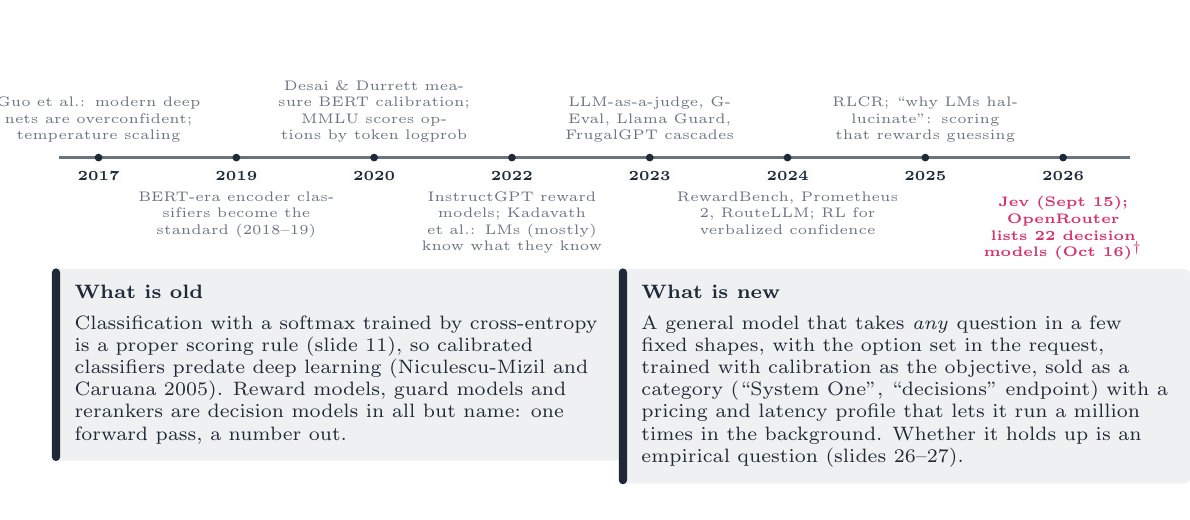
\begin{tikzpicture}
  \useasboundingbox (0,0) rectangle (14.4,5.9);
  \draw[muted,line width=0.8pt] (0.4,4.25) -- (14.0,4.25);
  \foreach \yr/\x in {2017/0.9,2019/2.65,2020/4.4,2022/6.15,2023/7.9,2024/9.65,2025/11.4,2026/13.15}{
    \fill[ink] (\x,4.25) circle (1.4pt);
    \node[font=\tiny\bfseries,text=ink,fill=paper,inner sep=1pt] at (\x,4.02) {\yr};}
  % above the line: even events; below: odd events
  \node[lab,anchor=south,text width=3.0cm,align=center,font=\tiny] at (0.9,4.38) {Guo et al.: modern deep nets are overconfident; temperature scaling};
  \node[lab,anchor=north,text width=3.0cm,align=center,font=\tiny] at (2.65,3.88) {BERT-era encoder classifiers become the standard (2018--19)};
  \node[lab,anchor=south,text width=3.0cm,align=center,font=\tiny] at (4.4,4.38) {Desai \& Durrett measure BERT calibration; MMLU scores options by token logprob};
  \node[lab,anchor=north,text width=3.0cm,align=center,font=\tiny] at (6.15,3.88) {InstructGPT reward models; Kadavath et al.: LMs (mostly) know what they know};
  \node[lab,anchor=south,text width=3.0cm,align=center,font=\tiny] at (7.9,4.38) {LLM-as-a-judge, G-Eval, Llama Guard, FrugalGPT cascades};
  \node[lab,anchor=north,text width=3.0cm,align=center,font=\tiny] at (9.65,3.88) {RewardBench, Prometheus 2, RouteLLM; RL for verbalized confidence};
  \node[lab,anchor=south,text width=3.0cm,align=center,font=\tiny] at (11.4,4.38) {RLCR; ``why LMs hallucinate'': scoring that rewards guessing};
  \node[anchor=north,text width=2.4cm,align=center,font=\tiny\bfseries,text=outc] at (13.15,3.88) {Jev (Sept 15); OpenRouter lists 22 decision models (Oct 16)$^\dagger$};
  \bgpanels{0.3}{2.85}{6.7cm}{What is old}{%
    Classification with a softmax trained by cross-entropy is a proper
    scoring rule (slide 11), so calibrated classifiers predate deep
    learning (Niculescu-Mizil and Caruana 2005). Reward models, guard
    models and rerankers are decision models in all but name: one
    forward pass, a number out.}
  \bgpanels{7.5}{2.85}{6.7cm}{What is new}{%
    A general model that takes \emph{any} question in a few fixed shapes,
    with the option set in the request, trained with calibration as the
    objective, sold as a category (``System One'', ``decisions'' endpoint)
    with a pricing and latency profile that lets it run a million times
    in the background. Whether it holds up is an empirical question
    (slides 26--27).}
\end{tikzpicture}
\end{frame}

% ---------------------------------------------------------------- 5
\stage{2}
\begin{frame}{Four primitives: choice, score, noul, box}
\framesubtitle{Every question has a fixed answer shape; the shape decides what comes back and what confidence means.}
\centering
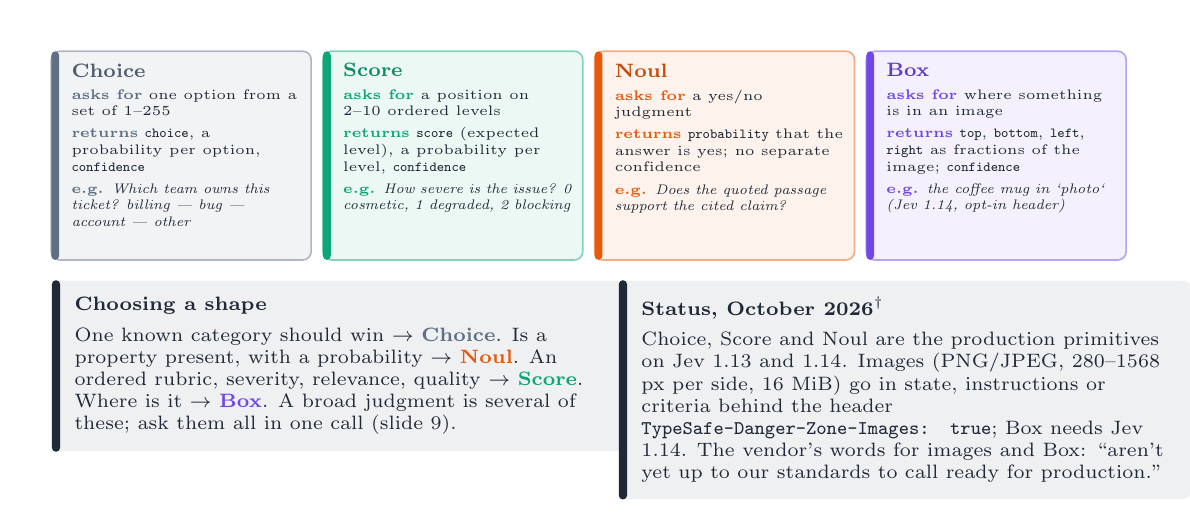
\begin{tikzpicture}
  \useasboundingbox (0,0) rectangle (14.4,5.9);
  \foreach \x/\c/\ttl/\asks/\ret/\ex in {
      0.3/tok/{Choice}/{one option from a set of 1--255}/{\texttt{choice}, a probability per option, \texttt{confidence}}/{Which team owns this ticket? billing | bug | account | other},
      3.75/emb/{Score}/{a position on 2--10 ordered levels}/{\texttt{score} (expected level), a probability per level, \texttt{confidence}}/{How severe is the issue? 0 cosmetic, 1 degraded, 2 blocking},
      7.2/attn/{Noul}/{a yes/no judgment}/{\texttt{probability} that the answer is yes; no separate confidence}/{Does the quoted passage support the cited claim?},
      10.65/posc/{Box}/{where something is in an image}/{\texttt{top}, \texttt{bottom}, \texttt{left}, \texttt{right} as fractions of the image; \texttt{confidence}}/{the coffee mug in `photo` (Jev 1.14, opt-in header)}}{
    \fill[\c!8,draw=\c!50,line width=0.6pt,rounded corners=3pt] (\x,2.95) rectangle (\x+3.3,5.6);
    \fill[\c,rounded corners=1.5pt] (\x,2.95) rectangle (\x+0.1,5.6);
    \node[anchor=north west,font=\scriptsize\bfseries,text=\c!85!black,inner sep=0] at (\x+0.25,5.45) {\ttl};
    \node[anchor=north west,font=\tiny,text=ink,inner sep=0,text width=2.9cm,align=flush left] at (\x+0.25,5.12) {%
      \hl{\c}{asks for} \asks\\[2pt]
      \hl{\c}{returns} \ret\\[2pt]
      \hl{\c}{e.g.} \emph{\ex}};}
  \bgpanels{0.3}{2.7}{6.7cm}{Choosing a shape}{%
    One known category should win $\to$ \hl{tok}{Choice}. Is a property
    present, with a probability $\to$ \hl{attn}{Noul}. An ordered rubric,
    severity, relevance, quality $\to$ \hl{emb}{Score}. Where is it
    $\to$ \hl{posc}{Box}. A broad judgment is several of these; ask them
    all in one call (slide 9).}
  \bgpanels{7.5}{2.7}{6.7cm}{Status, October 2026$^\dagger$}{%
    Choice, Score and Noul are the production primitives on Jev 1.13 and
    1.14. Images (PNG/JPEG, 280--1568 px per side, 16 MiB) go in state,
    instructions or criteria behind the header
    \texttt{TypeSafe-Danger-Zone-Images: true}; Box needs Jev 1.14.
    The vendor's words for images and Box: ``aren't yet up to our
    standards to call ready for production.''}
\end{tikzpicture}
\end{frame}

% ---------------------------------------------------------------- 6
\begin{frame}{Choice: a distribution over your options, plus one number}
\framesubtitle{The answer is the argmax; the probabilities are the real output; confidence is how far the top sits above an even split.}
\centering
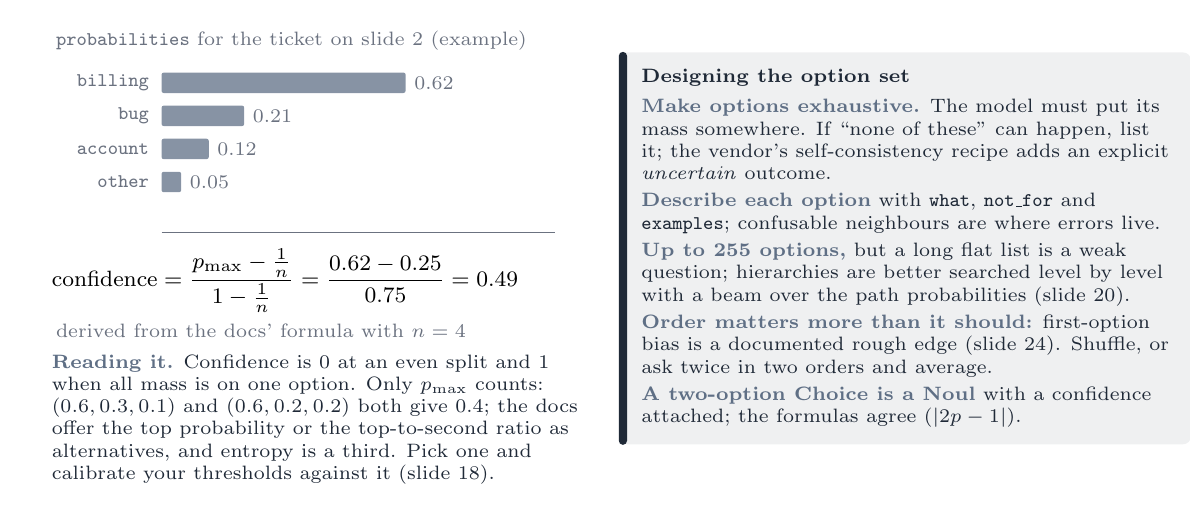
\begin{tikzpicture}
  \useasboundingbox (0,0) rectangle (14.4,5.9);
  \node[lab,anchor=south west] at (0.3,5.55) {\texttt{probabilities} for the ticket on slide 2 (example)};
  \foreach \i/\lab/\p in {0/billing/0.62,1/bug/0.21,2/account/0.12,3/other/0.05}{
    \node[lab,anchor=east,font=\scriptsize\ttfamily] at (1.6,{5.2-\i*0.42}) {\lab};
    \barh{1.7}{5.2-\i*0.42}{\p*5.0}{tok!75}
    \node[lab,anchor=west,font=\scriptsize] at ({1.75+\p*5.0},{5.2-\i*0.42}) {\p};}
  \draw[muted,line width=0.5pt] (1.7,3.3) -- (6.7,3.3);
  \node[anchor=north west,inner sep=0,font=\footnotesize] at (0.3,3.1) {%
    $\displaystyle\text{confidence}=\frac{p_{\max}-\tfrac1n}{1-\tfrac1n}
     =\frac{0.62-0.25}{0.75}=0.49$};
  \node[lab,anchor=north west] at (0.3,2.2) {derived from the docs' formula with $n=4$};
  \node[txt,anchor=north west,text width=6.7cm,font=\scriptsize] at (0.3,1.75) {%
    \hl{tok}{Reading it.} Confidence is 0 at an even split and 1 when all
    mass is on one option. Only $p_{\max}$ counts: $(0.6,0.3,0.1)$ and
    $(0.6,0.2,0.2)$ both give 0.4; the docs offer the top probability or
    the top-to-second ratio as alternatives, and entropy is a third. Pick
    one and calibrate your thresholds against it (slide 18).};
  \bgpanels{7.5}{5.6}{6.7cm}{Designing the option set}{%
    \hl{tok}{Make options exhaustive.} The model must put its mass
    somewhere. If ``none of these'' can happen, list it; the vendor's
    self-consistency recipe adds an explicit \emph{uncertain} outcome.\\[2pt]
    \hl{tok}{Describe each option} with \texttt{what}, \texttt{not\_for}
    and \texttt{examples}; confusable neighbours are where errors
    live.\\[2pt]
    \hl{tok}{Up to 255 options,} but a long flat list is a weak question;
    hierarchies are better searched level by level with a beam over the
    path probabilities (slide 20).\\[2pt]
    \hl{tok}{Order matters more than it should:} first-option bias is a
    documented rough edge (slide 24). Shuffle, or ask twice in two
    orders and average.\\[2pt]
    \hl{tok}{A two-option Choice is a Noul} with a confidence attached;
    the formulas agree ($|2p-1|$).}
\end{tikzpicture}
\end{frame}

% ---------------------------------------------------------------- 7
\begin{frame}{Score: ordered levels, an expected level, and a spread}
\framesubtitle{The score is the probability-weighted level, so it can sit between levels; confidence is how tight the mass is.}
\centering
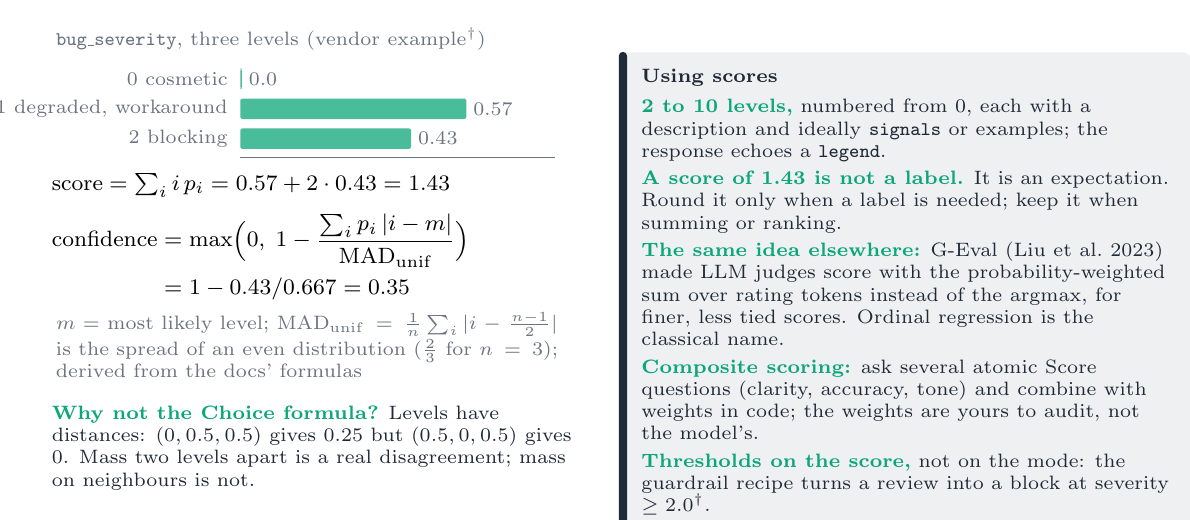
\begin{tikzpicture}
  \useasboundingbox (0,0) rectangle (14.4,5.9);
  \node[lab,anchor=south west] at (0.3,5.55) {\texttt{bug\_severity}, three levels (vendor example$^\dagger$)};
  \foreach \i/\lab/\p in {0/{0 cosmetic}/0.0,1/{1 degraded, workaround}/0.57,2/{2 blocking}/0.43}{
    \node[lab,anchor=east,font=\scriptsize] at (2.6,{5.25-\i*0.38}) {\lab};
    \barh{2.7}{5.25-\i*0.38}{\p*5.0+0.02}{emb!75}
    \node[lab,anchor=west,font=\scriptsize] at ({2.75+\p*5.0},{5.25-\i*0.38}) {\p};}
  \draw[muted,line width=0.5pt] (2.7,4.25) -- (6.7,4.25);
  \node[anchor=north west,inner sep=0,font=\footnotesize,align=left] at (0.3,4.05) {%
    $\text{score}=\sum_i i\,p_i = 0.57+2\cdot0.43 = 1.43$\\[5pt]
    $\displaystyle\text{confidence}=\max\Bigl(0,\;1-\frac{\sum_i p_i\,|i-m|}{\mathrm{MAD}_{\mathrm{unif}}}\Bigr)$\\[3pt]
    $\phantom{\text{confidence}}=1-0.43/0.667=0.35$};
  \node[lab,anchor=north west,text width=6.8cm] at (0.3,2.35) {$m$ = most likely level;
    $\mathrm{MAD}_{\mathrm{unif}}=\frac1n\sum_i|i-\frac{n-1}{2}|$ is the spread of an even
    distribution ($\tfrac23$ for $n=3$); derived from the docs' formulas};
  \node[txt,anchor=north west,text width=6.7cm,font=\scriptsize] at (0.3,1.1) {%
    \hl{emb}{Why not the Choice formula?} Levels have distances:
    $(0,0.5,0.5)$ gives 0.25 but $(0.5,0,0.5)$ gives 0. Mass two levels
    apart is a real disagreement; mass on neighbours is not.};
  \bgpanels{7.5}{5.6}{6.7cm}{Using scores}{%
    \hl{emb}{2 to 10 levels,} numbered from 0, each with a description
    and ideally \texttt{signals} or examples; the response echoes a
    \texttt{legend}.\\[2pt]
    \hl{emb}{A score of 1.43 is not a label.} It is an expectation. Round
    it only when a label is needed; keep it when summing or ranking.\\[2pt]
    \hl{emb}{The same idea elsewhere:} G-Eval (Liu et al.\ 2023) made
    LLM judges score with the probability-weighted sum over rating
    tokens instead of the argmax, for finer, less tied scores. Ordinal
    regression is the classical name.\\[2pt]
    \hl{emb}{Composite scoring:} ask several atomic Score questions
    (clarity, accuracy, tone) and combine with weights in code; the
    weights are yours to audit, not the model's.\\[2pt]
    \hl{emb}{Thresholds on the score,} not on the mode: the guardrail
    recipe turns a review into a block at severity $\geq 2.0$$^\dagger$.}
\end{tikzpicture}
\end{frame}

% ---------------------------------------------------------------- 8
\begin{frame}{Noul and Box: a single probability, and four edges}
\framesubtitle{Noul is the workhorse for verification and detection; Box is the first step outside text, and still a preview.}
\centering
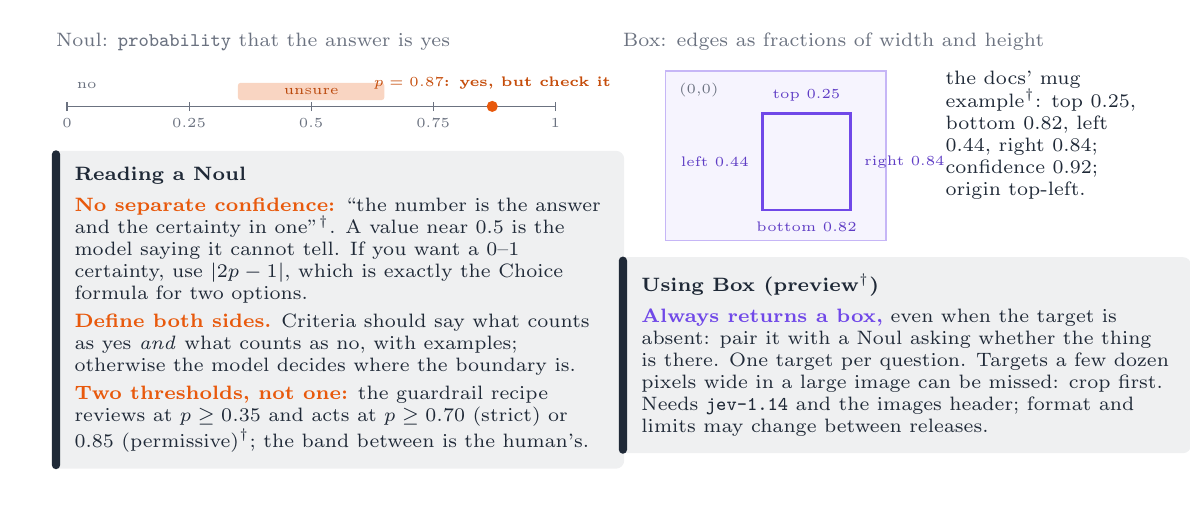
\begin{tikzpicture}
  \useasboundingbox (0,0) rectangle (14.4,5.9);
  % noul scale
  \node[lab,anchor=south west] at (0.3,5.55) {Noul: \texttt{probability} that the answer is yes};
  \draw[muted,line width=0.6pt] (0.5,4.9) -- (6.7,4.9);
  \foreach \x/\t in {0.5/0,2.05/0.25,3.6/0.5,5.15/0.75,6.7/1}{\draw[muted] (\x,4.84) -- (\x,4.96); \node[lab,anchor=north,font=\tiny] at (\x,4.8) {\t};}
  \fill[attn!25,rounded corners=1pt] (2.67,4.98) rectangle (4.53,5.2);
  \node[font=\tiny,text=attn!80!black] at (3.6,5.09) {unsure};
  \node[font=\tiny,text=muted,anchor=south west] at (0.5,5.0) {no};

  \fill[attn] (5.9,4.9) circle (2pt);
  \node[font=\tiny\bfseries,text=attn!85!black,anchor=south] at (5.9,5.0) {$p=0.87$: yes, but check it};
  \bgpanels{0.3}{4.35}{6.7cm}{Reading a Noul}{%
    \hl{attn}{No separate confidence:} ``the number is the answer and the
    certainty in one''$^\dagger$. A value near 0.5 is the model saying it
    cannot tell. If you want a 0--1 certainty, use $|2p-1|$, which is
    exactly the Choice formula for two options.\\[2pt]
    \hl{attn}{Define both sides.} Criteria should say what counts as
    yes \emph{and} what counts as no, with examples; otherwise the
    model decides where the boundary is.\\[2pt]
    \hl{attn}{Two thresholds, not one:} the guardrail recipe reviews at
    $p\geq0.35$ and acts at $p\geq0.70$ (strict) or 0.85
    (permissive)$^\dagger$; the band between is the human's.}
  % box illustration
  \node[lab,anchor=south west] at (7.5,5.55) {Box: edges as fractions of width and height};
  \fill[posc!6,draw=posc!40,line width=0.5pt] (8.1,3.2) rectangle (10.9,5.35);
  \draw[posc,line width=0.9pt] ({8.1+0.44*2.8},{5.35-0.82*2.15}) rectangle ({8.1+0.84*2.8},{5.35-0.25*2.15});
  \node[font=\tiny,text=posc!85!black,anchor=south] at ({8.1+0.64*2.8},{5.35-0.25*2.15+0.03}) {top 0.25};
  \node[font=\tiny,text=posc!85!black,anchor=north] at ({8.1+0.64*2.8},{5.35-0.82*2.15-0.03}) {bottom 0.82};
  \node[font=\tiny,text=posc!85!black,anchor=east] at ({8.1+0.44*2.8-0.05},{5.35-0.535*2.15}) {left 0.44};
  \node[font=\tiny,text=posc!85!black,anchor=west] at ({8.1+0.84*2.8+0.05},{5.35-0.535*2.15}) {right 0.84};
  \node[font=\tiny,text=muted,anchor=north west] at (8.15,5.32) {(0,0)};
  \node[txt,anchor=north west,text width=2.6cm,font=\scriptsize] at (11.65,5.35) {%
    the docs' mug example$^\dagger$: top 0.25, bottom 0.82, left 0.44, right 0.84; confidence 0.92; origin top-left.};
  \bgpanels{7.5}{3.0}{6.7cm}{Using Box (preview$^\dagger$)}{%
    \hl{posc}{Always returns a box,} even when the target is absent: pair
    it with a Noul asking whether the thing is there. One target per
    question. Targets a few dozen pixels wide in a large image can be
    missed: crop first. Needs \texttt{jev-1.14} and the images header;
    format and limits may change between releases.}
\end{tikzpicture}
\end{frame}

% ---------------------------------------------------------------- 9
\begin{frame}{State and questions: facts go in, judgments are asked}
\framesubtitle{One request evaluates one state against many independent questions; batching costs nothing in accuracy.}
\centering
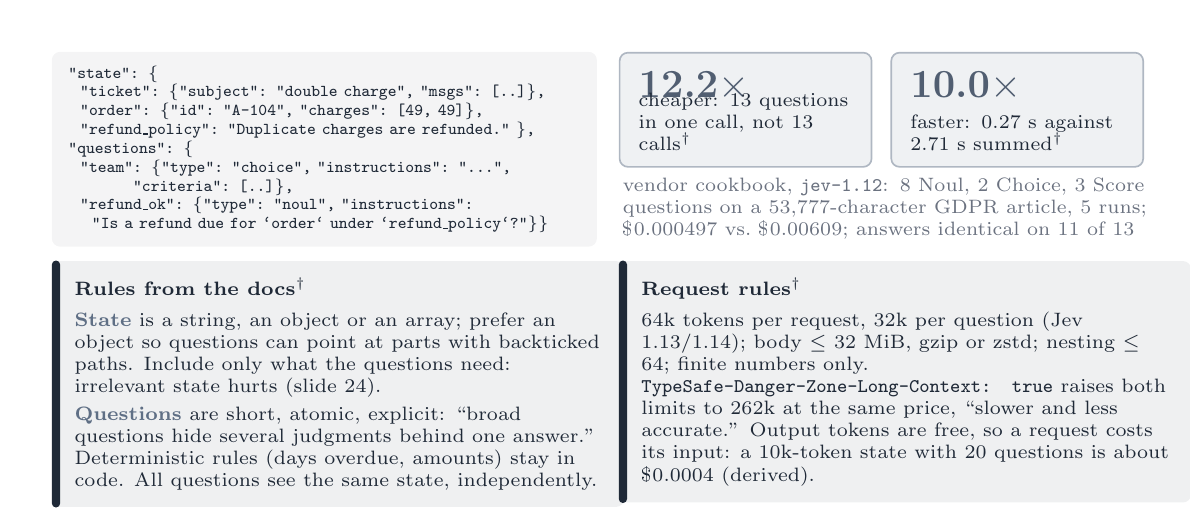
\begin{tikzpicture}
  \useasboundingbox (0,0) rectangle (14.4,5.9);
  \node[anchor=north west,inner sep=0,font=\ttfamily\fontsize{5.8}{6.8}\selectfont,text=ink,
        rounded corners=3pt,fill=ink!5,inner xsep=6pt,inner ysep=5pt,text width=6.5cm,align=left] at (0.3,5.6) {%
    "state": \{\\
    \ \ "ticket": \{"subject": "double charge", "msgs": [..]\},\\
    \ \ "order": \{"id": "A-104", "charges": [49, 49]\},\\
    \ \ "refund\_policy": "Duplicate charges are refunded." \},\\
    "questions": \{\\
    \ \ "team": \{"type": "choice", "instructions": "...",\\
    \ \ \ \ \ \ \ \ \ \ \ "criteria": [..]\},\\
    \ \ "refund\_ok": \{"type": "noul", "instructions":\\
    \ \ \ \ "Is a refund due for `order` under `refund\_policy`?"\}\}};
  \bgpanels{0.3}{2.95}{6.7cm}{Rules from the docs$^\dagger$}{%
    \hl{tok}{State} is a string, an object or an array; prefer an object
    so questions can point at parts with backticked paths. Include only
    what the questions need: irrelevant state hurts (slide 24).\\[2pt]
    \hl{tok}{Questions} are short, atomic, explicit: ``broad questions
    hide several judgments behind one answer.'' Deterministic rules
    (days overdue, amounts) stay in code. All questions see the same
    state, independently.}
  \stat{7.5}{5.6}{12.2$\times$}{cheaper: 13 questions in one call, not 13 calls$^\dagger$}{tok}
  \stat{10.95}{5.6}{10.0$\times$}{faster: 0.27 s against 2.71 s summed$^\dagger$}{tok}
  \node[lab,anchor=north west,text width=6.7cm] at (7.5,4.05) {vendor cookbook, \texttt{jev-1.12}: 8 Noul, 2 Choice, 3 Score questions on a 53{,}777-character GDPR article, 5 runs; \$0.000497 vs.\ \$0.00609; answers identical on 11 of 13};
  \bgpanels{7.5}{2.95}{6.7cm}{Request rules$^\dagger$}{%
    64k tokens per request, 32k per question (Jev 1.13/1.14); body
    $\leq$ 32 MiB, gzip or zstd; nesting $\leq$ 64; finite numbers only.
    \texttt{TypeSafe-Danger-Zone-Long-Context: true} raises both limits
    to 262k at the same price, ``slower and less accurate.'' Output
    tokens are free, so a request costs its input: a 10k-token state
    with 20 questions is about \$0.0004 (derived).}
\end{tikzpicture}
\end{frame}

% ---------------------------------------------------------------- 10
\stage{3}
\begin{frame}{Calibration: the probability has to mean something}
\framesubtitle{Of all the answers given with probability $p$, about a fraction $p$ should be right: a population property.}
\centering
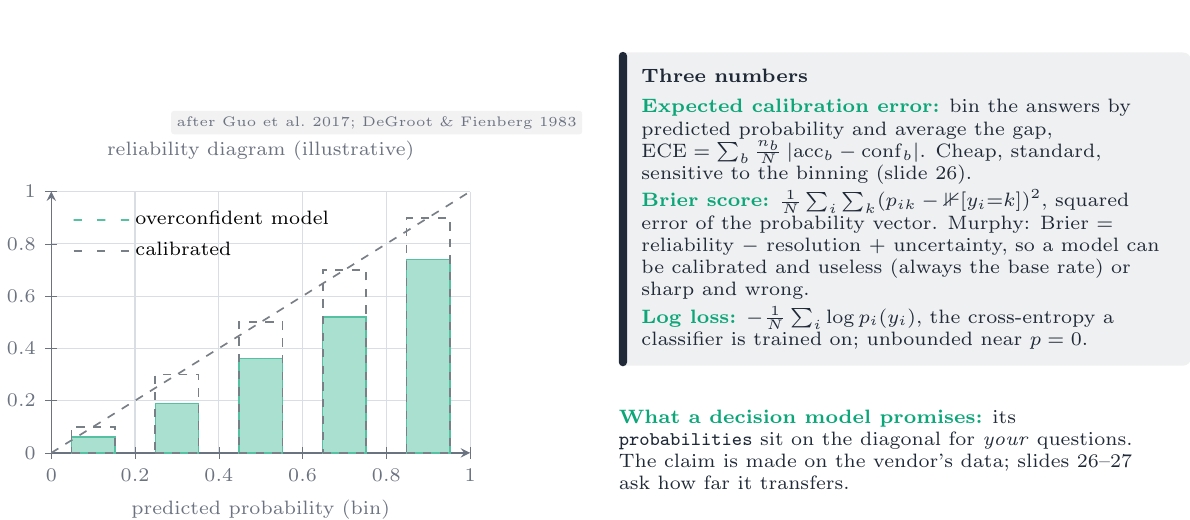
\begin{tikzpicture}
  \useasboundingbox (0,0) rectangle (14.4,5.9);
  \begin{scope}[shift={(0.3,0.5)}]
  \begin{axis}[lecture,width=6.9cm,height=4.9cm,xmin=0,xmax=1,ymin=0,ymax=1,
      xlabel={predicted probability (bin)},ylabel={fraction correct},
      xtick={0,0.2,...,1},ytick={0,0.2,...,1},
      legend pos=north west,legend style={at={(0.03,0.97)}},
      title style={font=\scriptsize,text=muted,at={(0.5,1.02)}},title={reliability diagram (illustrative)}]
    \addplot[ybar,bar width=0.55cm,fill=emb!35,draw=emb!70,line width=0.5pt] coordinates
      {(0.1,0.06) (0.3,0.19) (0.5,0.36) (0.7,0.52) (0.9,0.74)};
    \addlegendentry{overconfident model}
    \addplot[ybar,bar width=0.55cm,fill=none,draw=ink!60,line width=0.6pt,dashed] coordinates
      {(0.1,0.1) (0.3,0.3) (0.5,0.5) (0.7,0.7) (0.9,0.9)};
    \addlegendentry{calibrated}
    \addplot[ink!60,line width=0.6pt,dashed,domain=0:1] {x};
  \end{axis}
  \end{scope}
  \srctag{7.05}{4.85}{after Guo et al.\ 2017; DeGroot \& Fienberg 1983}
  \bgpanels{7.5}{5.6}{6.7cm}{Three numbers}{%
    \hl{emb}{Expected calibration error:} bin the answers by predicted
    probability and average the gap,
    $\mathrm{ECE}=\sum_b \frac{n_b}{N}\,|\mathrm{acc}_b-\mathrm{conf}_b|$.
    Cheap, standard, sensitive to the binning (slide 26).\\[2pt]
    \hl{emb}{Brier score:} $\frac1N\sum_i\sum_k (p_{ik}-\mathbb 1[y_i{=}k])^2$,
    squared error of the probability vector. Murphy: Brier $=$ reliability
    $-$ resolution $+$ uncertainty, so a model can be calibrated and
    useless (always the base rate) or sharp and wrong.\\[2pt]
    \hl{emb}{Log loss:} $-\frac1N\sum_i\log p_i(y_i)$, the cross-entropy a
    classifier is trained on; unbounded near $p=0$.}
  \node[txt,anchor=north west,text width=6.7cm,font=\scriptsize] at (7.5,1.05) {%
    \hl{emb}{What a decision model promises:} its \texttt{probabilities}
    sit on the diagonal for \emph{your} questions. The claim is made on
    the vendor's data; slides 26--27 ask how far it transfers.};
\end{tikzpicture}
\end{frame}

% ---------------------------------------------------------------- 11
\begin{frame}{Proper scoring rules make honesty the best policy}
\framesubtitle{Score the probability, not the guess: a strictly proper rule is optimized only by reporting the true belief.}
\centering
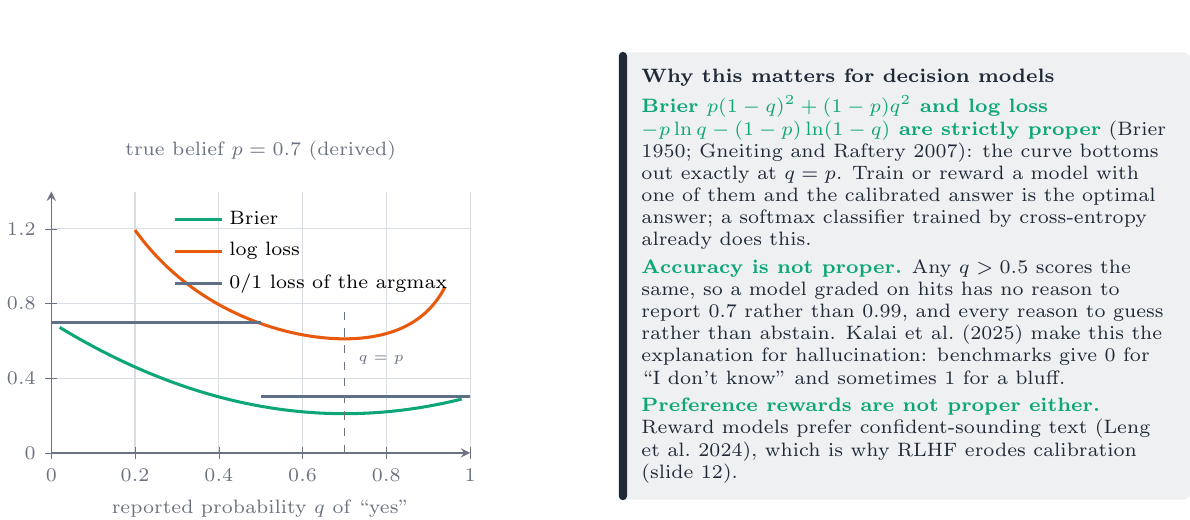
\begin{tikzpicture}
  \useasboundingbox (0,0) rectangle (14.4,5.9);
  \begin{scope}[shift={(0.3,0.5)}]
  \begin{axis}[lecture,width=6.9cm,height=4.9cm,xmin=0,xmax=1,ymin=0,ymax=1.4,
      xlabel={reported probability $q$ of ``yes''},ylabel={expected loss},
      xtick={0,0.2,...,1},ytick={0,0.4,0.8,1.2},
      legend pos=north east,legend style={at={(0.98,0.97)},anchor=north east},
      title style={font=\scriptsize,text=muted,at={(0.5,1.02)}},title={true belief $p=0.7$ (derived)}]
    \addplot[emb,line width=1.1pt,domain=0.02:0.98,samples=80] {0.7*(1-x)^2+0.3*x^2};
    \addlegendentry{Brier}
    \addplot[attn,line width=1.1pt,domain=0.2:0.94,samples=80] {-(0.7*ln(x)+0.3*ln(1-x))};
    \addlegendentry{log loss}
    \addplot[tok,line width=1.1pt,domain=0:0.5,samples=2] {0.7};
    \addplot[tok,line width=1.1pt,domain=0.5:1,samples=2] {0.3};
    \addlegendentry{0/1 loss of the argmax}
    \draw[muted,dashed] (axis cs:0.7,0) -- (axis cs:0.7,0.8);
    \node[font=\tiny,text=muted,anchor=west] at (axis cs:0.71,0.5) {$q=p$};
  \end{axis}
  \end{scope}
  \bgpanels{7.5}{5.6}{6.7cm}{Why this matters for decision models}{%
    \hl{emb}{Brier $p(1-q)^2+(1-p)q^2$ and log loss $-p\ln q-(1-p)\ln(1-q)$
    are strictly proper} (Brier 1950; Gneiting and Raftery 2007): the
    curve bottoms out exactly at $q=p$. Train or reward a model with one
    of them and the calibrated answer is the optimal answer; a softmax
    classifier trained by cross-entropy already does this.\\[2pt]
    \hl{emb}{Accuracy is not proper.} Any $q>0.5$ scores the same, so a
    model graded on hits has no reason to report 0.7 rather than 0.99,
    and every reason to guess rather than abstain. Kalai et al.\ (2025)
    make this the explanation for hallucination: benchmarks give 0 for
    ``I don't know'' and sometimes 1 for a bluff.\\[2pt]
    \hl{emb}{Preference rewards are not proper either.} Reward models
    prefer confident-sounding text (Leng et al.\ 2024), which is why
    RLHF erodes calibration (slide 12).}
\end{tikzpicture}
\end{frame}

% ---------------------------------------------------------------- 12
\begin{frame}{Do language models know what they know? Until post-training}
\framesubtitle{Base models are calibrated in the right format; preference tuning breaks it; asking in words helps but overshoots.}
\centering
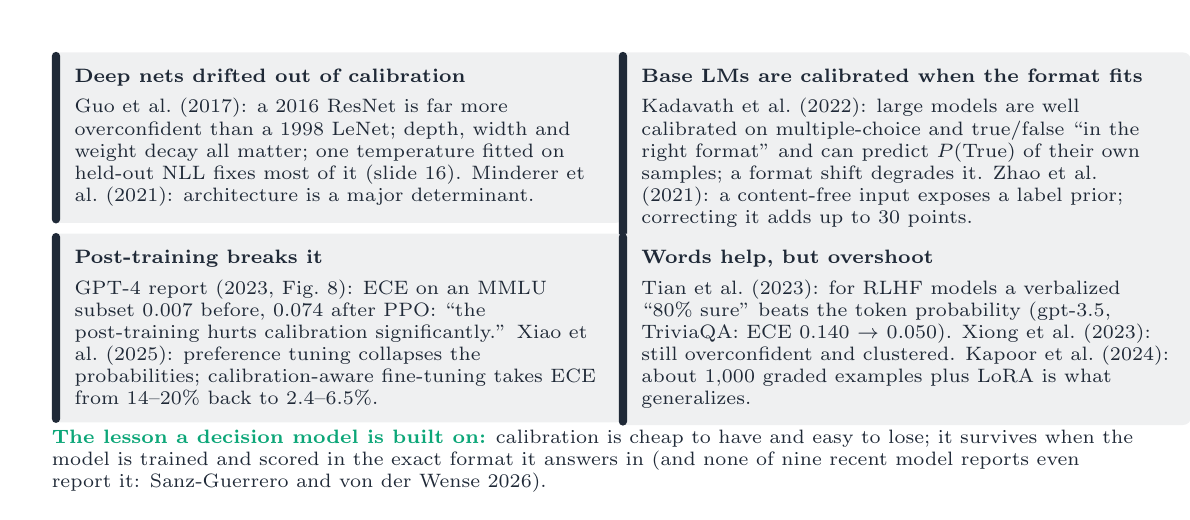
\begin{tikzpicture}
  \useasboundingbox (0,0) rectangle (14.4,5.9);
  \bgpanels{0.3}{5.6}{6.7cm}{Deep nets drifted out of calibration}{%
    Guo et al.\ (2017): a 2016 ResNet is far more overconfident than a
    1998 LeNet; depth, width and weight decay all matter; one temperature
    fitted on held-out NLL fixes most of it (slide 16). Minderer et al.\
    (2021): architecture is a major determinant.}
  \bgpanels{7.5}{5.6}{6.7cm}{Base LMs are calibrated when the format fits}{%
    Kadavath et al.\ (2022): large models are well calibrated on
    multiple-choice and true/false ``in the right format'' and can
    predict $P(\text{True})$ of their own samples; a format shift
    degrades it. Zhao et al.\ (2021): a content-free input exposes a
    label prior; correcting it adds up to 30 points.}
  \bgpanels{0.3}{3.3}{6.7cm}{Post-training breaks it}{%
    GPT-4 report (2023, Fig.\ 8): ECE on an MMLU subset 0.007 before,
    0.074 after PPO: ``the post-training hurts calibration
    significantly.'' Xiao et al.\ (2025): preference tuning collapses
    the probabilities; calibration-aware fine-tuning takes ECE from
    14--20\% back to 2.4--6.5\%.}
  \bgpanels{7.5}{3.3}{6.7cm}{Words help, but overshoot}{%
    Tian et al.\ (2023): for RLHF models a verbalized ``80\% sure'' beats
    the token probability (gpt-3.5, TriviaQA: ECE 0.140 $\to$ 0.050).
    Xiong et al.\ (2023): still overconfident and clustered. Kapoor et
    al.\ (2024): about 1{,}000 graded examples plus LoRA is what
    generalizes.}
  \node[txt,anchor=north west,text width=13.8cm,font=\scriptsize] at (0.3,0.8) {%
    \hl{emb}{The lesson a decision model is built on:} calibration is cheap
    to have and easy to lose; it survives when the model is trained and
    scored in the exact format it answers in (and none of nine recent
    model reports even report it: Sanz-Guerrero and von der Wense 2026).};
\end{tikzpicture}
\end{frame}

% ---------------------------------------------------------------- 13
\begin{frame}{Four ways to get a probability out of a language model}
\framesubtitle{Read the logits, ask in words, sample and count, or train a head. A decision model is the fourth, sold as a service.}
\centering
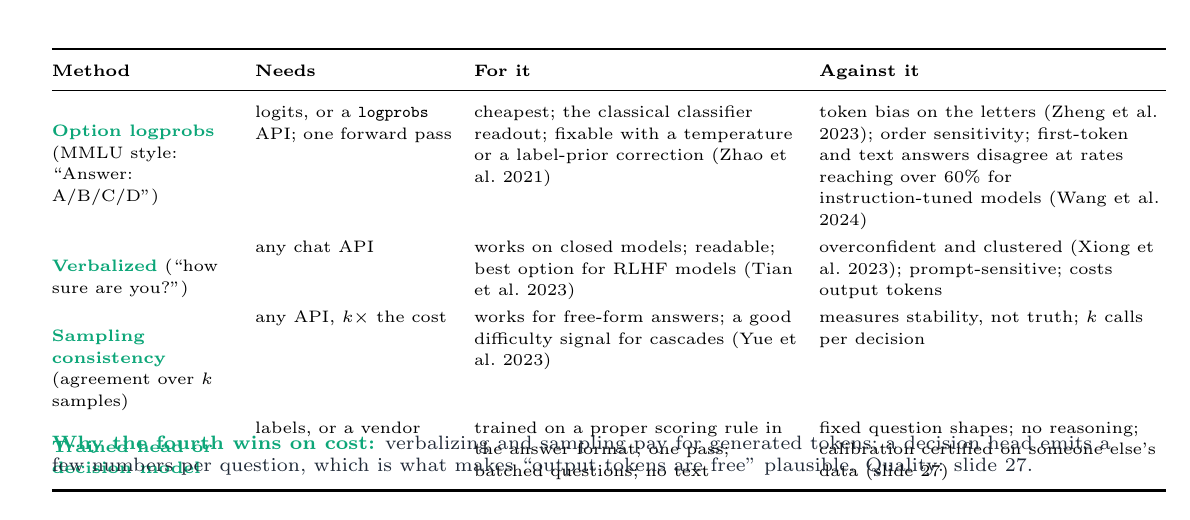
\begin{tikzpicture}
  \useasboundingbox (0,0) rectangle (14.4,5.9);
  \node[anchor=north west,inner sep=0,font=\fontsize{6.4}{7.8}\selectfont] at (0.3,5.65) {%
    \renewcommand{\arraystretch}{1.25}\setlength{\tabcolsep}{4pt}%
    \begin{tabular}{@{}>{\raggedright\arraybackslash}p{2.3cm}>{\raggedright\arraybackslash}p{2.5cm}>{\raggedright\arraybackslash}p{4.1cm}>{\raggedright\arraybackslash}p{4.4cm}@{}}
      \toprule
      \textbf{Method} & \textbf{Needs} & \textbf{For it} & \textbf{Against it}\\
      \midrule
      \hl{emb}{Option logprobs} (MMLU style: ``Answer: A/B/C/D'') & logits, or a \texttt{logprobs} API; one forward pass & cheapest; the classical classifier readout; fixable with a temperature or a label-prior correction (Zhao et al.\ 2021) & token bias on the letters (Zheng et al.\ 2023); order sensitivity; first-token and text answers disagree at rates reaching over 60\% for instruction-tuned models (Wang et al.\ 2024)\\
      \hl{emb}{Verbalized} (``how sure are you?'') & any chat API & works on closed models; readable; best option for RLHF models (Tian et al.\ 2023) & overconfident and clustered (Xiong et al.\ 2023); prompt-sensitive; costs output tokens\\
      \hl{emb}{Sampling consistency} (agreement over $k$ samples) & any API, $k\times$ the cost & works for free-form answers; a good difficulty signal for cascades (Yue et al.\ 2023) & measures stability, not truth; $k$ calls per decision\\
      \hl{emb}{Trained head or decision model} & labels, or a vendor & trained on a proper scoring rule in the answer format; one pass; batched questions; no text & fixed question shapes; no reasoning; calibration certified on someone else's data (slide 27)\\
      \bottomrule
    \end{tabular}};
  \node[txt,anchor=north west,text width=13.8cm,font=\scriptsize] at (0.3,0.72) {%
    \hl{emb}{Why the fourth wins on cost:} verbalizing and sampling pay for
    generated tokens; a decision head emits a few numbers per question, which
    is what makes ``output tokens are free'' plausible. Quality: slide 27.};
\end{tikzpicture}
\end{frame}

% ---------------------------------------------------------------- 14
\stage{4}
\begin{frame}{What is known about how a decision model is trained}
\framesubtitle{The vendor gives a name and a goal; the published recipes that match the goal all reward a proper scoring rule.}
\centering
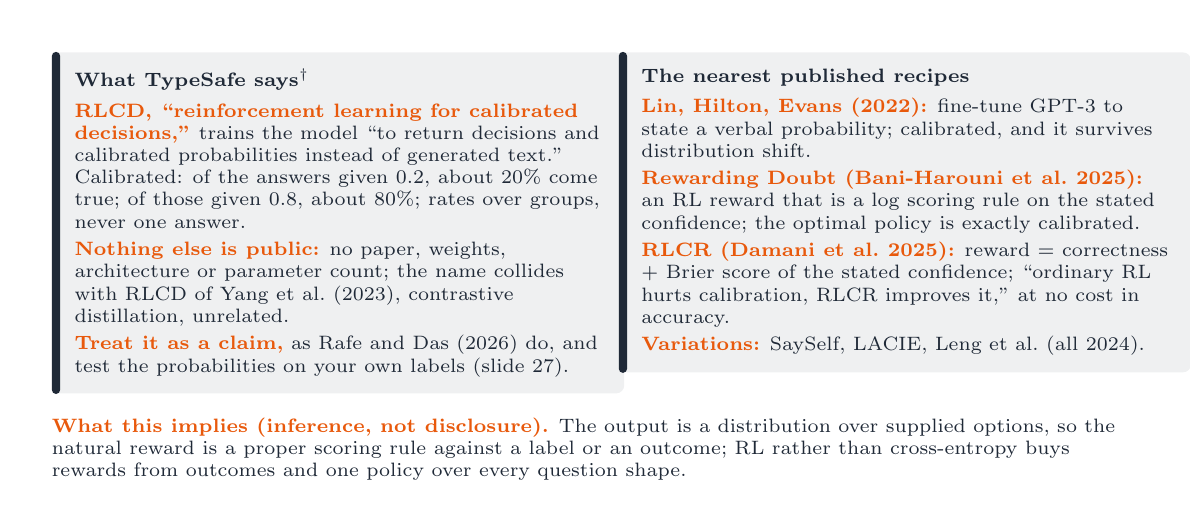
\begin{tikzpicture}
  \useasboundingbox (0,0) rectangle (14.4,5.9);
  \bgpanels{0.3}{5.6}{6.7cm}{What TypeSafe says$^\dagger$}{%
    \hl{attn}{RLCD, ``reinforcement learning for calibrated
    decisions,''} trains the model ``to return decisions and calibrated
    probabilities instead of generated text.'' Calibrated: of the
    answers given 0.2, about 20\% come true; of those given 0.8, about
    80\%; rates over groups, never one answer.\\[2pt]
    \hl{attn}{Nothing else is public:} no paper, weights, architecture
    or parameter count; the name collides with RLCD of Yang et al.\
    (2023), contrastive distillation, unrelated.\\[2pt]
    \hl{attn}{Treat it as a claim,} as Rafe and Das (2026) do, and test
    the probabilities on your own labels (slide 27).}
  \bgpanels{7.5}{5.6}{6.7cm}{The nearest published recipes}{%
    \hl{attn}{Lin, Hilton, Evans (2022):} fine-tune GPT-3 to state a
    verbal probability; calibrated, and it survives distribution shift.\\[2pt]
    \hl{attn}{Rewarding Doubt (Bani-Harouni et al.\ 2025):} an RL reward
    that is a log scoring rule on the stated confidence; the optimal
    policy is exactly calibrated.\\[2pt]
    \hl{attn}{RLCR (Damani et al.\ 2025):} reward $=$ correctness $+$
    Brier score of the stated confidence; ``ordinary RL hurts
    calibration, RLCR improves it,'' at no cost in accuracy.\\[2pt]
    \hl{attn}{Variations:} SaySelf, LACIE, Leng et al.\ (all 2024).}
  \node[txt,anchor=north west,text width=13.8cm,font=\scriptsize] at (0.3,0.95) {%
    \hl{attn}{What this implies (inference, not disclosure).} The output is a
    distribution over supplied options, so the natural reward is a proper
    scoring rule against a label or an outcome; RL rather than cross-entropy
    buys rewards from outcomes and one policy over every question shape.};
\end{tikzpicture}
\end{frame}

% ---------------------------------------------------------------- 15
\begin{frame}{RLHF, RLVR, RLCD: three objectives, three kinds of model}
\framesubtitle{What the signal is, what the policy emits, what gets rewarded, and what each one is known to get wrong.}
\centering
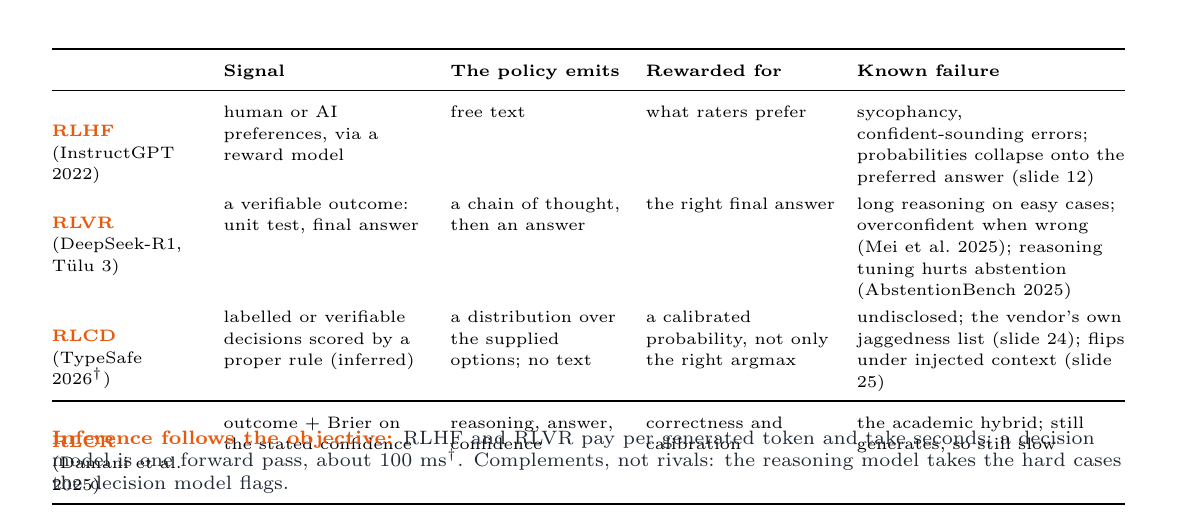
\begin{tikzpicture}
  \useasboundingbox (0,0) rectangle (14.4,5.9);
  \node[anchor=north west,inner sep=0,font=\fontsize{6.4}{7.8}\selectfont] at (0.3,5.65) {%
    \renewcommand{\arraystretch}{1.25}\setlength{\tabcolsep}{4pt}%
    \begin{tabular}{@{}>{\raggedright\arraybackslash}p{1.9cm}>{\raggedright\arraybackslash}p{2.6cm}>{\raggedright\arraybackslash}p{2.2cm}>{\raggedright\arraybackslash}p{2.4cm}>{\raggedright\arraybackslash}p{3.4cm}@{}}
      \toprule
      & \textbf{Signal} & \textbf{The policy emits} & \textbf{Rewarded for} & \textbf{Known failure}\\
      \midrule
      \hl{attn}{RLHF}\newline (InstructGPT 2022) & human or AI preferences, via a reward model & free text & what raters prefer & sycophancy, confident-sounding errors; probabilities collapse onto the preferred answer (slide 12)\\
      \hl{attn}{RLVR}\newline (DeepSeek-R1, T\"ulu 3) & a verifiable outcome: unit test, final answer & a chain of thought, then an answer & the right final answer & long reasoning on easy cases; overconfident when wrong (Mei et al.\ 2025); reasoning tuning hurts abstention (AbstentionBench 2025)\\
      \hl{attn}{RLCD}\newline (TypeSafe 2026$^\dagger$) & labelled or verifiable decisions scored by a proper rule (inferred) & a distribution over the supplied options; no text & a calibrated probability, not only the right argmax & undisclosed; the vendor's own jaggedness list (slide 24); flips under injected context (slide 25)\\
      \midrule
      \hl{attn}{RLCR}\newline (Damani et al.\ 2025) & outcome $+$ Brier on the stated confidence & reasoning, answer, confidence & correctness and calibration & the academic hybrid; still generates, so still slow\\
      \bottomrule
    \end{tabular}};
  \node[txt,anchor=north west,text width=13.8cm,font=\scriptsize] at (0.3,0.78) {%
    \hl{attn}{Inference follows the objective:} RLHF and RLVR pay per
    generated token and take seconds; a decision model is one forward
    pass, about 100 ms$^\dagger$. Complements, not rivals: the reasoning
    model takes the hard cases the decision model flags.};
\end{tikzpicture}
\end{frame}

% ---------------------------------------------------------------- 16
\begin{frame}{Calibration after the fact: temperature, Platt, isotonic}
\framesubtitle{One scalar fitted on a few hundred labelled examples repairs most miscalibration without touching the argmax.}
\centering
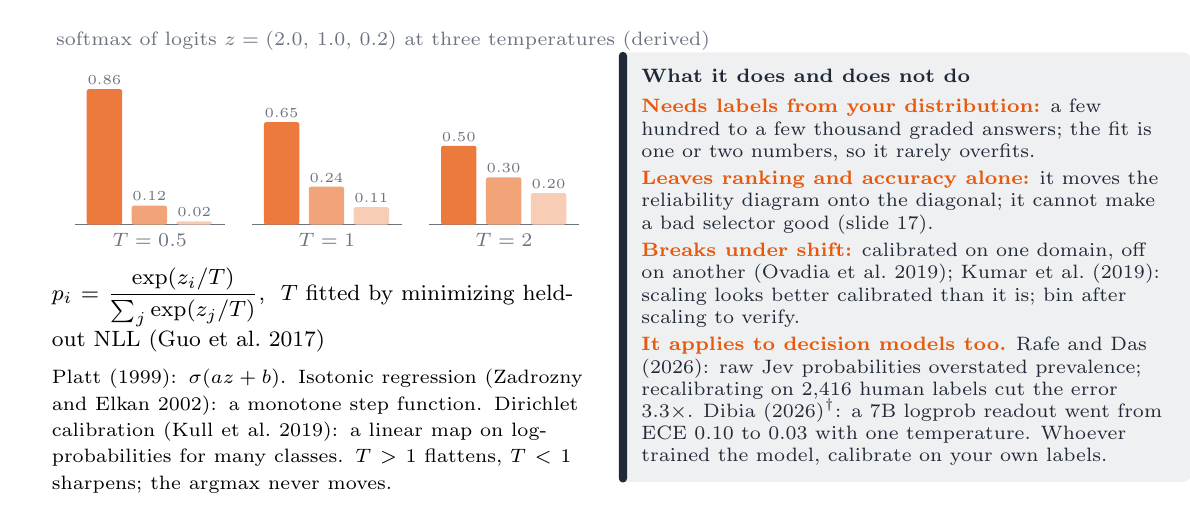
\begin{tikzpicture}
  \useasboundingbox (0,0) rectangle (14.4,5.9);
  \node[lab,anchor=south west] at (0.3,5.55) {softmax of logits $z=(2.0,\,1.0,\,0.2)$ at three temperatures (derived)};
  \foreach \g/\T/\pa/\pb/\pc in {0/{T=0.5}/0.86/0.12/0.02,1/{T=1}/0.65/0.24/0.11,2/{T=2}/0.50/0.30/0.20}{
    \begin{scope}[shift={(0.6+\g*2.25,3.4)}]
      \draw[muted,line width=0.5pt] (0,0) -- (1.9,0);
      \fill[attn!80,rounded corners=0.8pt] (0.15,0) rectangle ++(0.45,\pa*2.0);
      \fill[attn!55,rounded corners=0.8pt] (0.72,0) rectangle ++(0.45,\pb*2.0);
      \fill[attn!30,rounded corners=0.8pt] (1.29,0) rectangle ++(0.45,\pc*2.0);
      \node[lab,font=\tiny,anchor=south] at (0.375,\pa*2.0) {\pa};
      \node[lab,font=\tiny,anchor=south] at (0.945,\pb*2.0) {\pb};
      \node[lab,font=\tiny,anchor=south] at (1.515,\pc*2.0) {\pc};
      \node[lab,font=\scriptsize\bfseries,anchor=north] at (0.95,-0.05) {$\T$};
    \end{scope}}
  \node[anchor=north west,inner sep=0,font=\footnotesize,text width=6.8cm] at (0.3,2.85) {%
    $p_i=\dfrac{\exp(z_i/T)}{\sum_j\exp(z_j/T)}$, \ $T$ fitted by minimizing
    held-out NLL (Guo et al.\ 2017)\\[4pt]
    {\scriptsize Platt (1999): $\sigma(a z+b)$. Isotonic regression (Zadrozny and
    Elkan 2002): a monotone step function. Dirichlet calibration (Kull et
    al.\ 2019): a linear map on log-probabilities for many classes. $T>1$
    flattens, $T<1$ sharpens; the argmax never moves.}};
  \bgpanels{7.5}{5.6}{6.7cm}{What it does and does not do}{%
    \hl{attn}{Needs labels from your distribution:} a few hundred to a
    few thousand graded answers; the fit is one or two numbers, so it
    rarely overfits.\\[2pt]
    \hl{attn}{Leaves ranking and accuracy alone:} it moves the
    reliability diagram onto the diagonal; it cannot make a bad selector
    good (slide 17).\\[2pt]
    \hl{attn}{Breaks under shift:} calibrated on one domain, off on
    another (Ovadia et al.\ 2019); Kumar et al.\ (2019): scaling looks
    better calibrated than it is; bin after scaling to verify.\\[2pt]
    \hl{attn}{It applies to decision models too.} Rafe and Das (2026):
    raw Jev probabilities overstated prevalence; recalibrating on 2{,}416
    human labels cut the error 3.3$\times$. Dibia (2026)$^\dagger$: a
    7B logprob readout went from ECE 0.10 to 0.03 with one temperature.
    Whoever trained the model, calibrate on your own labels.}
\end{tikzpicture}
\end{frame}

% ---------------------------------------------------------------- 17
\stage{5}
\begin{frame}{Selective prediction: answer when sure, hand off the rest}
\framesubtitle{Sort decisions by confidence and stop answering below a threshold; error against coverage is the trade-off.}
\centering
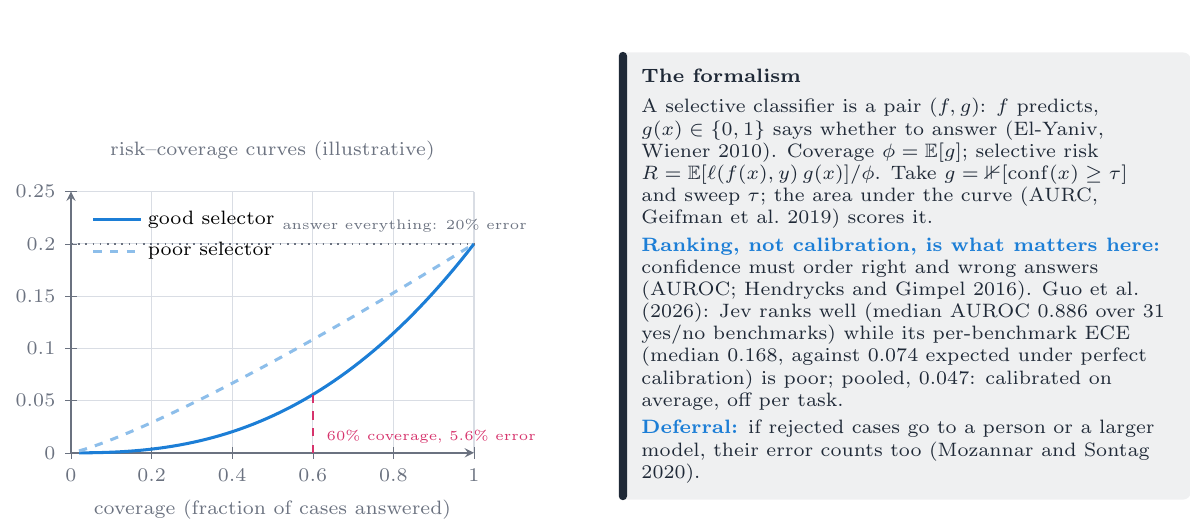
\begin{tikzpicture}
  \useasboundingbox (0,0) rectangle (14.4,5.9);
  \begin{scope}[shift={(0.55,0.5)}]
  \begin{axis}[lecture,width=6.7cm,height=4.9cm,xmin=0,xmax=1,ymin=0,ymax=0.25,
      xlabel={coverage (fraction of cases answered)},ylabel={selective risk (error rate)},
      xtick={0,0.2,...,1},ytick={0,0.05,...,0.25},
      y tick label style={/pgf/number format/fixed,/pgf/number format/precision=2},
      legend pos=north west,legend style={at={(0.03,0.97)},anchor=north west},
      title style={font=\scriptsize,text=muted,at={(0.5,1.02)}},title={risk--coverage curves (illustrative)}]
    \addplot[mlp,line width=1.1pt,domain=0.02:1,samples=60] {0.2*x^2.5};
    \addlegendentry{good selector}
    \addplot[mlp!50,line width=1.1pt,dashed,domain=0.02:1,samples=60] {0.2*x^1.2};
    \addlegendentry{poor selector}
    \addplot[muted,line width=0.6pt,dotted,domain=0:1] {0.2};
    \node[font=\tiny,text=muted,anchor=south west] at (axis cs:0.5,0.202) {answer everything: 20\% error};
    \draw[outc,line width=0.6pt,dashed] (axis cs:0.6,0) -- (axis cs:0.6,0.056);
    \node[font=\tiny,text=outc,anchor=south west] at (axis cs:0.61,0.0) {60\% coverage, 5.6\% error};
  \end{axis}
  \end{scope}
  \bgpanels{7.5}{5.6}{6.7cm}{The formalism}{%
    A selective classifier is a pair $(f,g)$: $f$ predicts, $g(x)\in\{0,1\}$
    says whether to answer (El-Yaniv, Wiener 2010). Coverage
    $\phi=\mathbb E[g]$; selective risk $R=\mathbb E[\ell(f(x),y)\,g(x)]/\phi$.
    Take $g=\mathbb 1[\mathrm{conf}(x)\geq\tau]$ and sweep $\tau$; the area
    under the curve (AURC, Geifman et al.\ 2019) scores it.\\[2pt]
    \hl{mlp}{Ranking, not calibration, is what matters here:} confidence
    must order right and wrong answers (AUROC; Hendrycks and Gimpel
    2016). Guo et al.\ (2026): Jev ranks well (median AUROC 0.886 over 31
    yes/no benchmarks) while its per-benchmark ECE (median 0.168, against
    0.074 expected under perfect calibration) is poor; pooled, 0.047:
    calibrated on average, off per task.\\[2pt]
    \hl{mlp}{Deferral:} if rejected cases go to a person or a larger
    model, their error counts too (Mozannar and Sontag 2020).}
\end{tikzpicture}
\end{frame}

% ---------------------------------------------------------------- 18
\begin{frame}{Thresholds are a cost decision, not a model setting}
\framesubtitle{A calibrated probability turns ``how sure must we be?'' into arithmetic on the cost of each kind of mistake.}
\centering
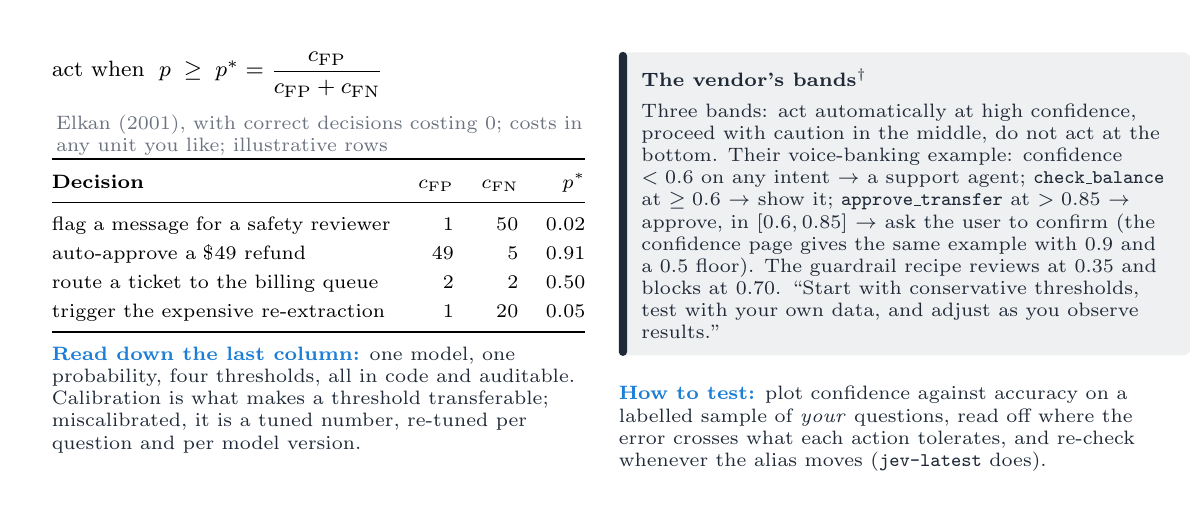
\begin{tikzpicture}
  \useasboundingbox (0,0) rectangle (14.4,5.9);
  \node[anchor=north west,inner sep=0,font=\footnotesize] at (0.3,5.6) {%
    act when $\;p \;\geq\; p^{*}=\dfrac{c_{\mathrm{FP}}}{c_{\mathrm{FP}}+c_{\mathrm{FN}}}$};
  \node[lab,anchor=north west,text width=6.9cm] at (0.3,4.85) {Elkan (2001), with correct decisions costing 0; costs in any unit you like; illustrative rows};
  \node[anchor=north west,inner sep=0,font=\fontsize{6.6}{8}\selectfont] at (0.3,4.25) {%
    \renewcommand{\arraystretch}{1.3}\setlength{\tabcolsep}{5pt}%
    \begin{tabular}{@{}>{\raggedright\arraybackslash}p{4.3cm}rrr@{}}
      \toprule
      \textbf{Decision} & $c_{\mathrm{FP}}$ & $c_{\mathrm{FN}}$ & $p^{*}$\\
      \midrule
      flag a message for a safety reviewer & 1 & 50 & 0.02\\
      auto-approve a \$49 refund & 49 & 5 & 0.91\\
      route a ticket to the billing queue & 2 & 2 & 0.50\\
      trigger the expensive re-extraction & 1 & 20 & 0.05\\
      \bottomrule
    \end{tabular}};
  \node[txt,anchor=north west,text width=6.8cm,font=\scriptsize] at (0.3,1.85) {%
    \hl{mlp}{Read down the last column:} one model, one probability, four
    thresholds, all in code and auditable. Calibration is what makes a
    threshold transferable; miscalibrated, it is a tuned number,
    re-tuned per question and per model version.};
  \bgpanels{7.5}{5.6}{6.7cm}{The vendor's bands$^\dagger$}{%
    Three bands: act automatically at high confidence, proceed with
    caution in the middle, do not act at the bottom. Their voice-banking
    example: confidence $<0.6$ on any intent $\to$ a support agent;
    \texttt{check\_balance} at $\geq0.6$ $\to$ show it;
    \texttt{approve\_transfer} at $>0.85$ $\to$ approve, in $[0.6,0.85]$
    $\to$ ask the user to confirm (the confidence page gives the same
    example with 0.9 and a 0.5 floor). The guardrail recipe reviews at
    0.35 and blocks at 0.70. ``Start with
    conservative thresholds, test with your own data, and adjust as you
    observe results.''}
  \node[txt,anchor=north west,text width=6.7cm,font=\scriptsize] at (7.5,1.35) {%
    \hl{mlp}{How to test:} plot confidence against accuracy on a
    labelled sample of \emph{your} questions, read off where the error
    crosses what each action tolerates, and re-check whenever the alias
    moves (\texttt{jev-latest} does).};
\end{tikzpicture}
\end{frame}

% ---------------------------------------------------------------- 19
\begin{frame}{Conformal prediction: sets with a coverage guarantee}
\framesubtitle{From any probability vector to a set that contains the right answer $1-\alpha$ of the time, with no model assumptions.}
\centering
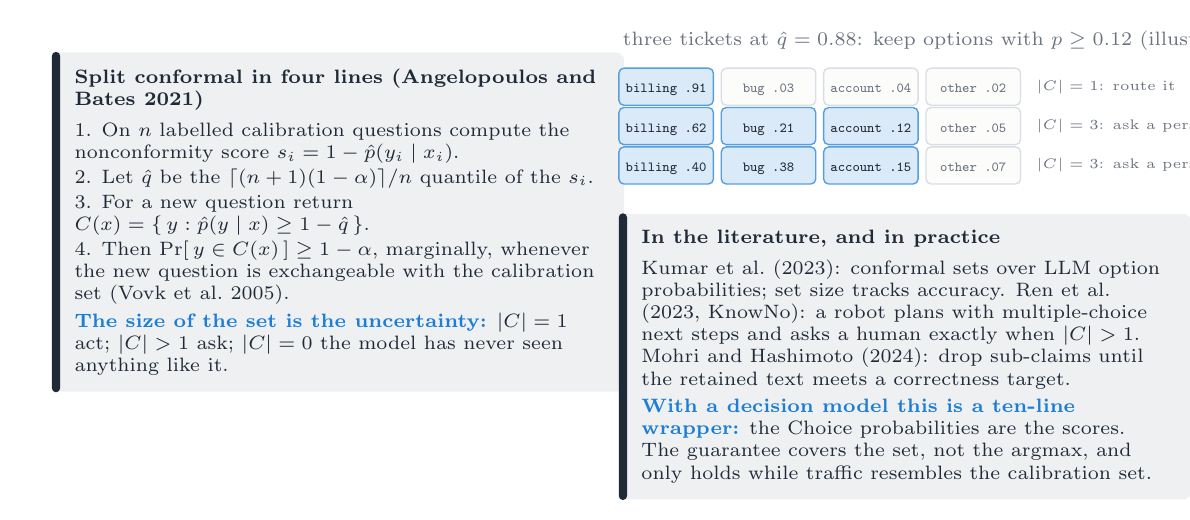
\begin{tikzpicture}
  \useasboundingbox (0,0) rectangle (14.4,5.9);
  \bgpanels{0.3}{5.6}{6.7cm}{Split conformal in four lines (Angelopoulos and Bates 2021)}{%
    1. On $n$ labelled calibration questions compute the nonconformity
    score $s_i = 1-\hat p(y_i\mid x_i)$.\\[1pt]
    2. Let $\hat q$ be the $\lceil (n+1)(1-\alpha)\rceil/n$ quantile of the
    $s_i$.\\[1pt]
    3. For a new question return $C(x)=\{\,y : \hat p(y\mid x)\geq 1-\hat q\,\}$.\\[1pt]
    4. Then $\Pr[\,y\in C(x)\,]\geq 1-\alpha$, marginally, whenever the new
    question is exchangeable with the calibration set (Vovk et al.\
    2005).\\[2pt]
    \hl{mlp}{The size of the set is the uncertainty:} $|C|=1$ act;
    $|C|>1$ ask; $|C|=0$ the model has never seen anything like it.}
  \node[lab,anchor=south west] at (7.5,5.55) {three tickets at $\hat q=0.88$: keep options with $p\geq0.12$ (illustrative)};
  \foreach \r/\pa/\pb/\pc/\pd/\ka/\kb/\kc/\kd/\verdict in {
      0/.91/.03/.04/.02/1/0/0/0/{$|C|=1$: route it},
      1/.62/.21/.12/.05/1/1/1/0/{$|C|=3$: ask a person},
      2/.40/.38/.15/.07/1/1/1/0/{$|C|=3$: ask a person}}{
    \foreach \j/\lab/\p/\k in {0/billing/\pa/\ka,1/bug/\pb/\kb,2/account/\pc/\kc,3/other/\pd/\kd}{
      \ifnum\k=1
        \node[cchip=mlp,anchor=west,font=\ttfamily\tiny,minimum width=1.2cm,inner xsep=2pt] at ({7.5+\j*1.3},{5.15-\r*0.5}) {\lab\ \p};
      \else
        \node[chip,anchor=west,font=\ttfamily\tiny,minimum width=1.2cm,inner xsep=2pt,fill=paper,draw=hair,text=muted] at ({7.5+\j*1.3},{5.15-\r*0.5}) {\lab\ \p};
      \fi}
    \node[lab,anchor=west,font=\tiny] at (12.75,{5.15-\r*0.5}) {\verdict};}
  \bgpanels{7.5}{3.55}{6.7cm}{In the literature, and in practice}{%
    Kumar et al.\ (2023): conformal sets over LLM option probabilities;
    set size tracks accuracy. Ren et al.\ (2023, KnowNo): a robot plans
    with multiple-choice next steps and asks a human exactly when
    $|C|>1$. Mohri and Hashimoto (2024): drop sub-claims until the
    retained text meets a correctness target.\\[2pt]
    \hl{mlp}{With a decision model this is a ten-line wrapper:} the Choice
    probabilities are the scores. The guarantee covers the set, not the
    argmax, and only holds while traffic resembles the calibration set.}
\end{tikzpicture}
\end{frame}

% ---------------------------------------------------------------- 20
\begin{frame}{Cascades and fan-out: the cheap model decides who pays}
\framesubtitle{A small calibrated model in front of a large one, firing it only when flagged; and many questions asked in one pass.}
\centering
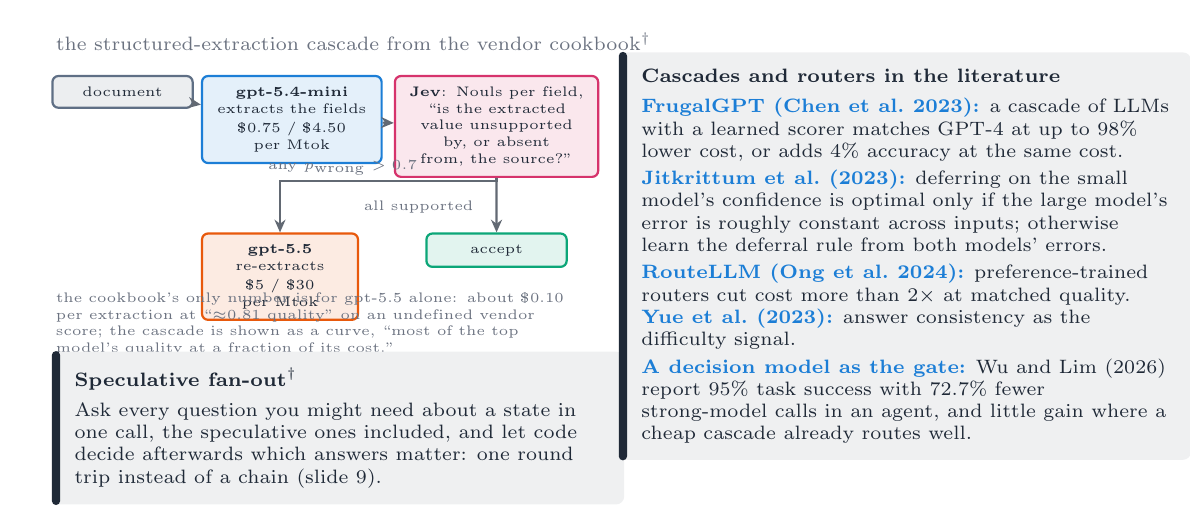
\begin{tikzpicture}
  \useasboundingbox (0,0) rectangle (14.4,5.9);
  % cascade diagram (vendor cookbook)
  \node[lab,anchor=south west] at (0.3,5.55) {the structured-extraction cascade from the vendor cookbook$^\dagger$};
  \node[comp=tok,anchor=north west,text width=1.5cm,font=\tiny] (d) at (0.3,5.3) {document};
  \node[comp=mlp,anchor=north west,text width=2.0cm,font=\tiny] (s1) at (2.2,5.3) {\textbf{gpt-5.4-mini} extracts the fields\\[1pt]\$0.75 / \$4.50 per Mtok};
  \node[comp=outc,anchor=north west,text width=2.3cm,font=\tiny] (v) at (4.65,5.3) {\textbf{Jev}: Nouls per field, ``is the extracted value unsupported by, or absent from, the source?''};
  \node[comp=attn,anchor=north west,text width=1.7cm,font=\tiny] (s2) at (2.2,3.3) {\textbf{gpt-5.5} re-extracts\\[1pt]\$5 / \$30 per Mtok};
  \node[comp=emb,anchor=north west,text width=1.5cm,font=\tiny] (ok) at (5.05,3.3) {accept};
  \draw[flow] (d) -- (s1); \draw[flow] (s1) -- (v);
  \draw[flow] (v.south) -- (v.south |- 0,3.95) -- (s2.north |- 0,3.95) -- (s2.north);
  \node[lab,font=\tiny,anchor=south] at (4.0,3.97) {any $p_{\mathrm{wrong}}>0.7$};
  \draw[flow] (v.south) -- (ok.north);
  \node[lab,font=\tiny,anchor=east] at (5.72,3.62) {all supported};
  \node[lab,anchor=north west,text width=6.7cm,font=\tiny] at (0.3,2.6) {the cookbook's only number is for gpt-5.5 alone: about \$0.10 per extraction at ``$\approx$0.81 quality'' on an undefined vendor score; the cascade is shown as a curve, ``most of the top model's quality at a fraction of its cost.''};
  \bgpanels{0.3}{1.8}{6.7cm}{Speculative fan-out$^\dagger$}{%
    Ask every question you might need about a state in one call, the
    speculative ones included, and let code decide afterwards which
    answers matter: one round trip instead of a chain (slide 9).}
  \bgpanels{7.5}{5.6}{6.7cm}{Cascades and routers in the literature}{%
    \hl{mlp}{FrugalGPT (Chen et al.\ 2023):} a cascade of LLMs with a
    learned scorer matches GPT-4 at up to 98\% lower cost, or adds 4\%
    accuracy at the same cost.\\[2pt]
    \hl{mlp}{Jitkrittum et al.\ (2023):} deferring on the small model's
    confidence is optimal only if the large model's error is roughly
    constant across inputs; otherwise learn the deferral rule from both
    models' errors.\\[2pt]
    \hl{mlp}{RouteLLM (Ong et al.\ 2024):} preference-trained routers cut
    cost more than 2$\times$ at matched quality. \hl{mlp}{Yue et al.\
    (2023):} answer consistency as the difficulty signal.\\[2pt]
    \hl{mlp}{A decision model as the gate:} Wu and Lim (2026) report 95\%
    task success with 72.7\% fewer strong-model calls in an agent, and
    little gain where a cheap cascade already routes well.}
\end{tikzpicture}
\end{frame}

% ---------------------------------------------------------------- 21
\stage{6}
\begin{frame}{Jev: the product that named the category}
\framesubtitle{Five weeks old on the day of this lecture; a price, a latency and a request volume that explain the attention.}
\centering
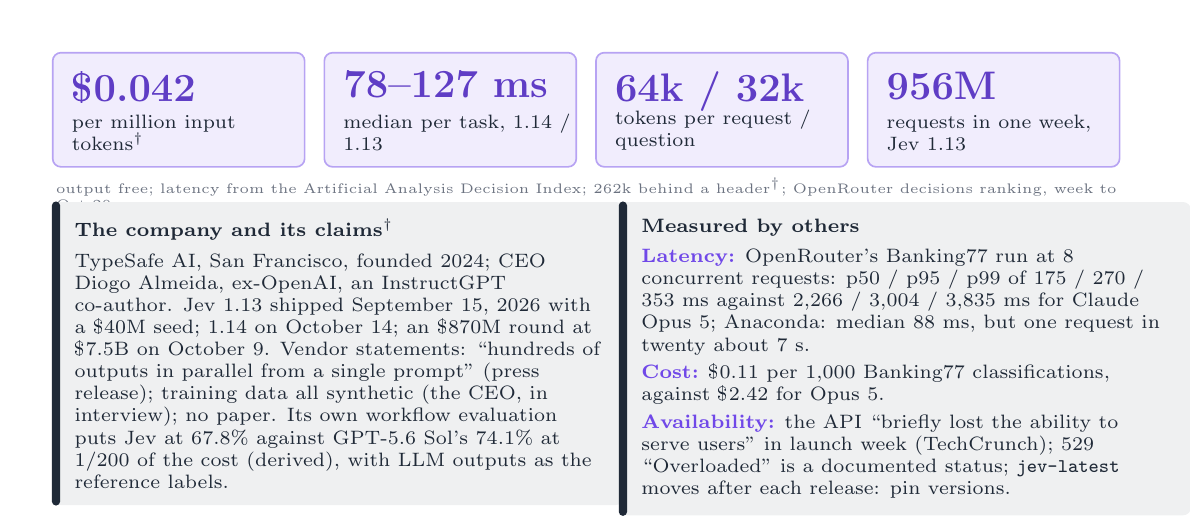
\begin{tikzpicture}
  \useasboundingbox (0,0) rectangle (14.4,5.9);
  \stat{0.3}{5.6}{\$0.042}{per million input tokens$^\dagger$}{posc}
  \stat{3.75}{5.6}{78--127 ms}{median per task, 1.14 / 1.13}{posc}
  \stat{7.2}{5.6}{64k / 32k}{tokens per request / question}{posc}
  \stat{10.65}{5.6}{956M}{requests in one week, Jev 1.13}{posc}
  \node[lab,anchor=north west,text width=13.8cm,font=\tiny] at (0.3,4.05) {output free; latency from the Artificial Analysis Decision Index; 262k behind a header$^\dagger$; OpenRouter decisions ranking, week to Oct 20};
  \bgpanels{0.3}{3.7}{6.7cm}{The company and its claims$^\dagger$}{%
    TypeSafe AI, San Francisco, founded 2024; CEO Diogo Almeida,
    ex-OpenAI, an InstructGPT co-author. Jev 1.13 shipped September 15,
    2026 with a \$40M seed; 1.14 on October 14; an \$870M round at \$7.5B
    on October 9. Vendor statements: ``hundreds of outputs in parallel
    from a single prompt'' (press release); training data all synthetic
    (the CEO, in interview); no paper. Its own workflow evaluation puts
    Jev at 67.8\% against GPT-5.6 Sol's 74.1\% at 1/200 of the cost
    (derived), with LLM outputs as the reference labels.}
  \bgpanels{7.5}{3.7}{6.7cm}{Measured by others}{%
    \hl{posc}{Latency:} OpenRouter's Banking77 run at 8 concurrent
    requests: p50 / p95 / p99 of 175 / 270 / 353 ms against 2{,}266 /
    3{,}004 / 3{,}835 ms for Claude Opus 5; Anaconda: median 88 ms, but
    one request in twenty about 7 s.\\[2pt]
    \hl{posc}{Cost:} \$0.11 per 1{,}000 Banking77 classifications, against
    \$2.42 for Opus 5.\\[2pt]
    \hl{posc}{Availability:} the API ``briefly lost the ability to serve
    users'' in launch week (TechCrunch); 529 ``Overloaded'' is a
    documented status; \texttt{jev-latest} moves after each release:
    pin versions.}
\end{tikzpicture}
\end{frame}

% ---------------------------------------------------------------- 22
\begin{frame}{The landscape, October 2026: one category, many insides}
\framesubtitle{OpenRouter's guide lists 22 decision models from 13 makers (Oct 16); the open ones show how different the insides are.}
\centering
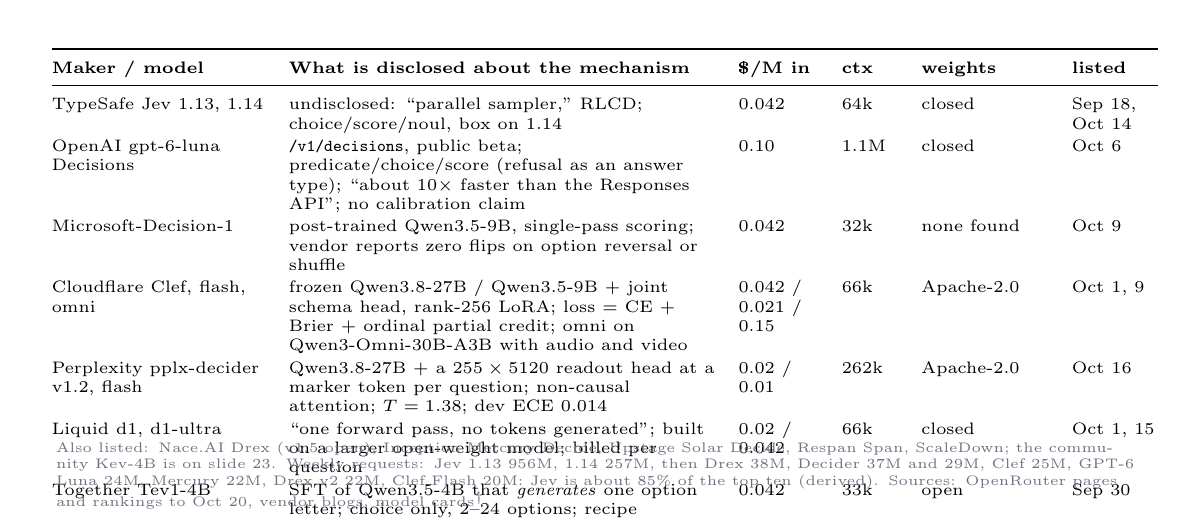
\begin{tikzpicture}
  \useasboundingbox (0,0) rectangle (14.4,5.9);
  \node[anchor=north west,inner sep=0,font=\fontsize{5.9}{7.0}\selectfont] at (0.3,5.65) {%
    \renewcommand{\arraystretch}{1.15}\setlength{\tabcolsep}{3pt}%
    \begin{tabular}{@{}>{\raggedright\arraybackslash}p{2.8cm}>{\raggedright\arraybackslash}p{5.5cm}>{\raggedright\arraybackslash}p{1.1cm}>{\raggedright\arraybackslash}p{0.8cm}>{\raggedright\arraybackslash}p{1.7cm}>{\raggedright\arraybackslash}p{1.1cm}@{}}
      \toprule
      \textbf{Maker / model} & \textbf{What is disclosed about the mechanism} & \textbf{\$/M in} & \textbf{ctx} & \textbf{weights} & \textbf{listed}\\
      \midrule
      TypeSafe Jev 1.13, 1.14 & undisclosed: ``parallel sampler,'' RLCD; choice/score/noul, box on 1.14 & 0.042 & 64k & closed & Sep 18, Oct 14\\
      OpenAI gpt-6-luna Decisions & \texttt{/v1/decisions}, public beta; predicate/choice/score (refusal as an answer type); ``about 10$\times$ faster than the Responses API''; no calibration claim & 0.10 & 1.1M & closed & Oct 6\\
      Microsoft-Decision-1 & post-trained Qwen3.5-9B, single-pass scoring; vendor reports zero flips on option reversal or shuffle & 0.042 & 32k & none found & Oct 9\\
      Cloudflare Clef, flash, omni & frozen Qwen3.8-27B / Qwen3.5-9B $+$ joint schema head, rank-256 LoRA; loss $=$ CE $+$ Brier $+$ ordinal partial credit; omni on Qwen3-Omni-30B-A3B with audio and video & 0.042 / 0.021 / 0.15 & 66k & Apache-2.0 & Oct 1, 9\\
      Perplexity pplx-decider v1.2, flash & Qwen3.8-27B $+$ a $255\times5120$ readout head at a marker token per question; non-causal attention; $T=1.38$; dev ECE 0.014 & 0.02 / 0.01 & 262k & Apache-2.0 & Oct 16\\
      Liquid d1, d1-ultra & ``one forward pass, no tokens generated''; built on a larger open-weight model; billed per question & 0.02 / 0.042 & 66k & closed & Oct 1, 15\\
      Together Tev1-4B & SFT of Qwen3.5-4B that \emph{generates} one option letter; choice only, 2--24 options; recipe published & 0.042 & 33k & open & Sep 30\\
      \bottomrule
    \end{tabular}};
  \node[lab,anchor=north west,text width=13.8cm,font=\tiny] at (0.3,0.7) {Also listed: Nace.AI Drex (v1.5 open), Inception Mercury Decide, Upstage Solar Decide, Respan Span, ScaleDown; the community Kev-4B is on slide 23. Weekly requests: Jev 1.13 956M, 1.14 257M, then Drex 38M, Decider 37M and 29M, Clef 25M, GPT-6 Luna 24M, Mercury 22M, Drex v2 22M, Clef Flash 20M: Jev is about 85\% of the top ten (derived). Sources: OpenRouter pages and rankings to Oct 20, vendor blogs, model cards$^\dagger$.};
\end{tikzpicture}
\end{frame}

% ---------------------------------------------------------------- 23
\begin{frame}{Open weights: four ways to build one, all on Hugging Face}
\framesubtitle{Read the letters, generate a letter, bolt a head onto a frozen LLM, or fine-tune an encoder; llama.cpp serves them all.}
\centering
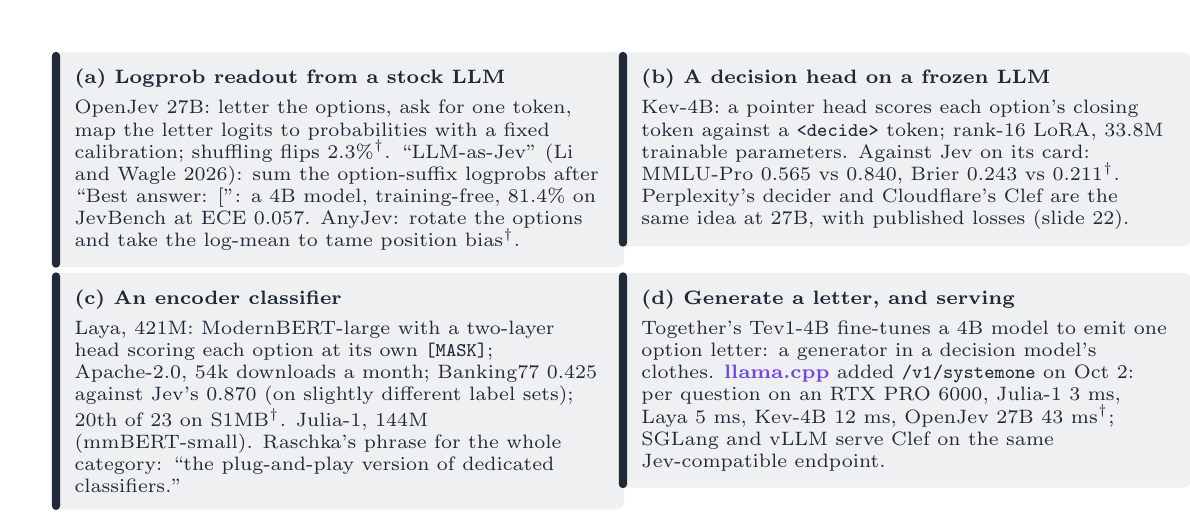
\begin{tikzpicture}
  \useasboundingbox (0,0) rectangle (14.4,5.9);
  \bgpanels{0.3}{5.6}{6.7cm}{(a) Logprob readout from a stock LLM}{%
    OpenJev 27B: letter the options, ask for one token, map the letter
    logits to probabilities with a fixed calibration; shuffling flips
    2.3\%$^\dagger$. ``LLM-as-Jev'' (Li and Wagle 2026): sum the
    option-suffix logprobs after ``Best answer: ['': a 4B model,
    training-free, 81.4\% on JevBench at ECE 0.057. AnyJev: rotate the
    options and take the log-mean to tame position bias$^\dagger$.}
  \bgpanels{7.5}{5.6}{6.7cm}{(b) A decision head on a frozen LLM}{%
    Kev-4B: a pointer head scores each option's closing token against a
    \texttt{<decide>} token; rank-16 LoRA, 33.8M trainable parameters.
    Against Jev on its card: MMLU-Pro 0.565 vs 0.840, Brier 0.243 vs
    0.211$^\dagger$. Perplexity's decider and
    Cloudflare's Clef are the same idea at 27B, with published losses
    (slide 22).}
  \bgpanels{0.3}{2.8}{6.7cm}{(c) An encoder classifier}{%
    Laya, 421M: ModernBERT-large with a two-layer head scoring each
    option at its own \texttt{[MASK]}; Apache-2.0, 54k downloads a
    month; Banking77 0.425 against Jev's 0.870 (on slightly different
    label sets); 20th of 23 on S1MB$^\dagger$. Julia-1, 144M (mmBERT-small). Raschka's phrase for
    the whole category: ``the plug-and-play version of dedicated
    classifiers.''}
  \bgpanels{7.5}{2.8}{6.7cm}{(d) Generate a letter, and serving}{%
    Together's Tev1-4B fine-tunes a 4B model to emit one option letter:
    a generator in a decision model's clothes.
    \hl{posc}{llama.cpp} added \texttt{/v1/systemone} on Oct 2: per
    question on an RTX PRO 6000, Julia-1 3 ms, Laya 5 ms, Kev-4B 12 ms,
    OpenJev 27B 43 ms$^\dagger$; SGLang and vLLM serve Clef on the same
    Jev-compatible endpoint.}
\end{tikzpicture}
\end{frame}

% ---------------------------------------------------------------- 24
\stage{7}
\begin{frame}{Jaggedness: where a decision model is rough}
\framesubtitle{The vendor publishes its own list; independent tests confirm it and add wording sensitivity.}
\centering
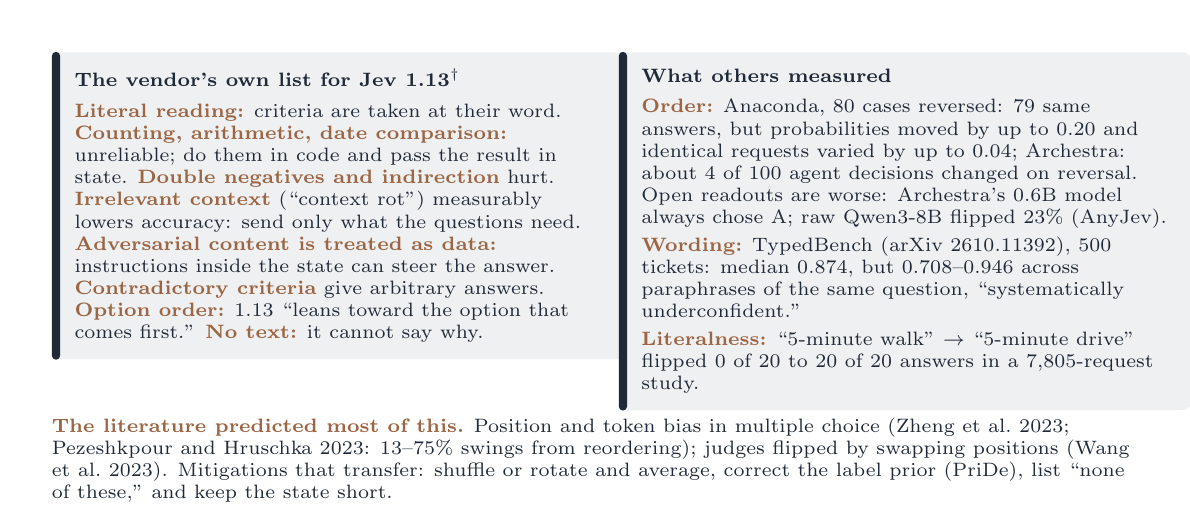
\begin{tikzpicture}
  \useasboundingbox (0,0) rectangle (14.4,5.9);
  \bgpanels{0.3}{5.6}{6.7cm}{The vendor's own list for Jev 1.13$^\dagger$}{%
    \hl{trn}{Literal reading:} criteria are taken at their word.
    \hl{trn}{Counting, arithmetic, date comparison:} unreliable; do them
    in code and pass the result in state.
    \hl{trn}{Double negatives and indirection} hurt.
    \hl{trn}{Irrelevant context} (``context rot'') measurably lowers
    accuracy: send only what the questions need.
    \hl{trn}{Adversarial content is treated as data:} instructions
    inside the state can steer the answer.
    \hl{trn}{Contradictory criteria} give arbitrary answers.
    \hl{trn}{Option order:} 1.13 ``leans toward the option that comes
    first.''
    \hl{trn}{No text:} it cannot say why.}
  \bgpanels{7.5}{5.6}{6.7cm}{What others measured}{%
    \hl{trn}{Order:} Anaconda, 80 cases reversed: 79 same answers, but
    probabilities moved by up to 0.20 and identical requests varied by
    up to 0.04; Archestra: about 4 of 100 agent decisions changed on
    reversal. Open readouts are worse: Archestra's 0.6B model always
    chose A; raw Qwen3-8B flipped 23\% (AnyJev).\\[2pt]
    \hl{trn}{Wording:} TypedBench (arXiv 2610.11392), 500 tickets: median
    0.874, but 0.708--0.946 across paraphrases of the same question,
    ``systematically underconfident.''\\[2pt]
    \hl{trn}{Literalness:} ``5-minute walk'' $\to$ ``5-minute drive''
    flipped 0 of 20 to 20 of 20 answers in a 7{,}805-request study.}
  \node[txt,anchor=north west,text width=13.8cm,font=\scriptsize] at (0.3,0.95) {%
    \hl{trn}{The literature predicted most of this.} Position and token
    bias in multiple choice (Zheng et al.\ 2023; Pezeshkpour and Hruschka
    2023: 13--75\% swings from reordering); judges flipped by swapping
    positions (Wang et al.\ 2023). Mitigations that transfer: shuffle or
    rotate and average, correct the label prior (PriDe), list ``none of
    these,'' and keep the state short.};
\end{tikzpicture}
\end{frame}

% ---------------------------------------------------------------- 25
\begin{frame}{What a calibrated probability cannot tell you}
\framesubtitle{Calibration is about a population of questions; the state may be written by an adversary; the label is not the outcome.}
\centering
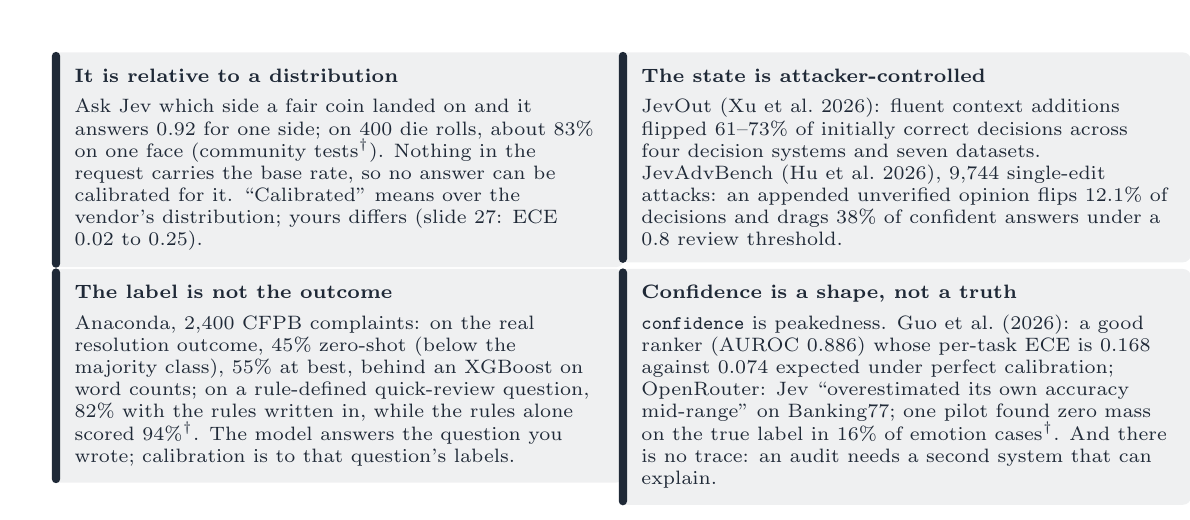
\begin{tikzpicture}
  \useasboundingbox (0,0) rectangle (14.4,5.9);
  \bgpanels{0.3}{5.6}{6.7cm}{It is relative to a distribution}{%
    Ask Jev which side a fair coin landed on and it answers 0.92 for one
    side; on 400 die rolls, about 83\% on one face (community
    tests$^\dagger$). Nothing in the request carries the base rate, so no
    answer can be calibrated for it. ``Calibrated'' means over the
    vendor's distribution; yours differs (slide 27: ECE 0.02 to 0.25).}
  \bgpanels{7.5}{5.6}{6.7cm}{The state is attacker-controlled}{%
    JevOut (Xu et al.\ 2026): fluent context additions flipped 61--73\% of
    initially correct decisions across four decision systems and seven
    datasets. JevAdvBench (Hu et al.\ 2026), 9{,}744 single-edit
    attacks: an appended unverified opinion flips 12.1\% of decisions
    and drags 38\% of confident answers under a 0.8 review threshold.}
  \bgpanels{0.3}{2.85}{6.7cm}{The label is not the outcome}{%
    Anaconda, 2{,}400 CFPB complaints: on the real resolution outcome,
    45\% zero-shot (below the majority class), 55\% at best, behind an
    XGBoost on word counts; on a rule-defined quick-review question, 82\%
    with the rules written in, while the rules alone scored
    94\%$^\dagger$. The model answers the question you wrote;
    calibration is to that question's labels.}
  \bgpanels{7.5}{2.85}{6.7cm}{Confidence is a shape, not a truth}{%
    \texttt{confidence} is peakedness. Guo et al.\ (2026): a good ranker
    (AUROC 0.886) whose per-task ECE is 0.168 against 0.074 expected
    under perfect calibration; OpenRouter: Jev
    ``overestimated its own accuracy mid-range'' on Banking77; one pilot
    found zero mass on the true label in 16\% of emotion
    cases$^\dagger$. And there is no trace: an audit needs a second
    system that can explain.}
\end{tikzpicture}
\end{frame}

% ---------------------------------------------------------------- 26
\stage{8}
\begin{frame}{Evaluating a decision model: six questions, six numbers}
\framesubtitle{Accuracy alone is the wrong test for a model whose product is a probability; test the probability and the selector.}
\centering
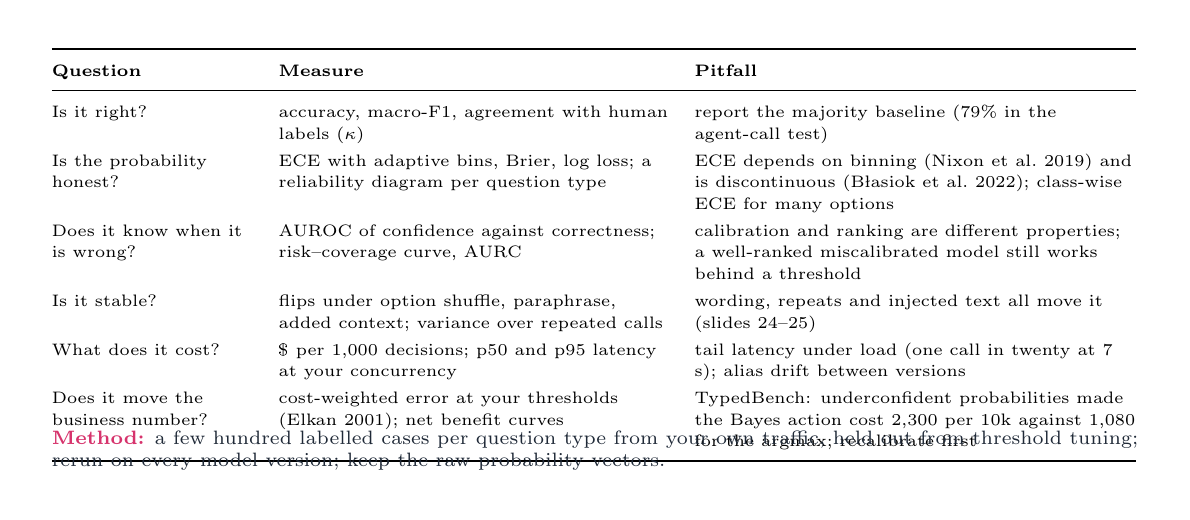
\begin{tikzpicture}
  \useasboundingbox (0,0) rectangle (14.4,5.9);
  \node[anchor=north west,inner sep=0,font=\fontsize{6.4}{7.8}\selectfont] at (0.3,5.65) {%
    \renewcommand{\arraystretch}{1.25}\setlength{\tabcolsep}{4pt}%
    \begin{tabular}{@{}>{\raggedright\arraybackslash}p{2.6cm}>{\raggedright\arraybackslash}p{5.0cm}>{\raggedright\arraybackslash}p{5.6cm}@{}}
      \toprule
      \textbf{Question} & \textbf{Measure} & \textbf{Pitfall}\\
      \midrule
      Is it right? & accuracy, macro-F1, agreement with human labels ($\kappa$) & report the majority baseline (79\% in the agent-call test)\\
      Is the probability honest? & ECE with adaptive bins, Brier, log loss; a reliability diagram per question type & ECE depends on binning (Nixon et al.\ 2019) and is discontinuous (B\l{}asiok et al.\ 2022); class-wise ECE for many options\\
      Does it know when it is wrong? & AUROC of confidence against correctness; risk--coverage curve, AURC & calibration and ranking are different properties; a well-ranked miscalibrated model still works behind a threshold\\
      Is it stable? & flips under option shuffle, paraphrase, added context; variance over repeated calls & wording, repeats and injected text all move it (slides 24--25)\\
      What does it cost? & \$ per 1{,}000 decisions; p50 and p95 latency at your concurrency & tail latency under load (one call in twenty at 7 s); alias drift between versions\\
      Does it move the business number? & cost-weighted error at your thresholds (Elkan 2001); net benefit curves & TypedBench: underconfident probabilities made the Bayes action cost 2{,}300 per 10k against 1{,}080 for the argmax; recalibrate first\\
      \bottomrule
    \end{tabular}};
  \node[txt,anchor=north west,text width=13.8cm,font=\scriptsize] at (0.3,0.78) {%
    \hl{outc}{Method:} a few hundred labelled cases per question type from
    your own traffic, held out from threshold tuning; rerun on every model
    version; keep the raw probability vectors.};
\end{tikzpicture}
\end{frame}

% ---------------------------------------------------------------- 27
\begin{frame}{What the independent evidence says, five weeks in}
\framesubtitle{Strong and cheap at discrimination, a few points under the best generators, calibration that depends on the task.}
\centering
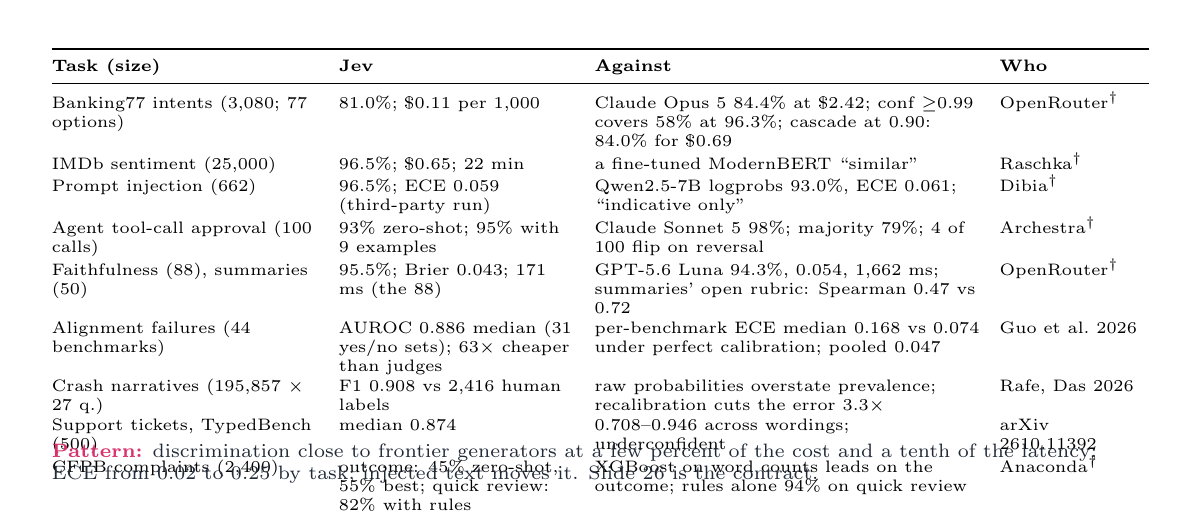
\begin{tikzpicture}
  \useasboundingbox (0,0) rectangle (14.4,5.9);
  \node[anchor=north west,inner sep=0,font=\fontsize{5.8}{6.9}\selectfont] at (0.3,5.65) {%
    \renewcommand{\arraystretch}{1.05}\setlength{\tabcolsep}{3.5pt}%
    \begin{tabular}{@{}>{\raggedright\arraybackslash}p{3.4cm}>{\raggedright\arraybackslash}p{3.0cm}>{\raggedright\arraybackslash}p{4.9cm}>{\raggedright\arraybackslash}p{1.9cm}@{}}
      \toprule
      \textbf{Task (size)} & \textbf{Jev} & \textbf{Against} & \textbf{Who}\\
      \midrule
      Banking77 intents (3{,}080; 77 options) & 81.0\%; \$0.11 per 1{,}000 & Claude Opus 5 84.4\% at \$2.42; conf $\geq$0.99 covers 58\% at 96.3\%; cascade at 0.90: 84.0\% for \$0.69 & OpenRouter$^\dagger$\\
      IMDb sentiment (25{,}000) & 96.5\%; \$0.65; 22 min & a fine-tuned ModernBERT ``similar'' & Raschka$^\dagger$\\
      Prompt injection (662) & 96.5\%; ECE 0.059 (third-party run) & Qwen2.5-7B logprobs 93.0\%, ECE 0.061; ``indicative only'' & Dibia$^\dagger$\\
      Agent tool-call approval (100 calls) & 93\% zero-shot; 95\% with 9 examples & Claude Sonnet 5 98\%; majority 79\%; 4 of 100 flip on reversal & Archestra$^\dagger$\\
      Faithfulness (88), summaries (50) & 95.5\%; Brier 0.043; 171 ms (the 88) & GPT-5.6 Luna 94.3\%, 0.054, 1{,}662 ms; summaries' open rubric: Spearman 0.47 vs 0.72 & OpenRouter$^\dagger$\\
      Alignment failures (44 benchmarks) & AUROC 0.886 median (31 yes/no sets); 63$\times$ cheaper than judges & per-benchmark ECE median 0.168 vs 0.074 under perfect calibration; pooled 0.047 & Guo et al.\ 2026\\
      Crash narratives (195{,}857 $\times$ 27 q.) & F1 0.908 vs 2{,}416 human labels & raw probabilities overstate prevalence; recalibration cuts the error 3.3$\times$ & Rafe, Das 2026\\
      Support tickets, TypedBench (500) & median 0.874 & 0.708--0.946 across wordings; underconfident & arXiv 2610.11392\\
      CFPB complaints (2{,}400) & outcome: 45\% zero-shot, 55\% best; quick review: 82\% with rules & XGBoost on word counts leads on the outcome; rules alone 94\% on quick review & Anaconda$^\dagger$\\
      \bottomrule
    \end{tabular}};
  \node[txt,anchor=north west,text width=13.8cm,font=\scriptsize] at (0.3,0.62) {%
    \hl{outc}{Pattern:} discrimination close to frontier generators at a few
    percent of the cost and a tenth of the latency; ECE from 0.02 to 0.25 by
    task; injected text moves it. Slide 26 is the contract.};
\end{tikzpicture}
\end{frame}

% ---------------------------------------------------------------- 28
\stage{9}
\begin{frame}{One decision, as it goes over the wire}
\framesubtitle{A coding agent asks whether to run a shell command: two Nouls, a Score, a deny-list in front, and thresholds in code.}
\centering
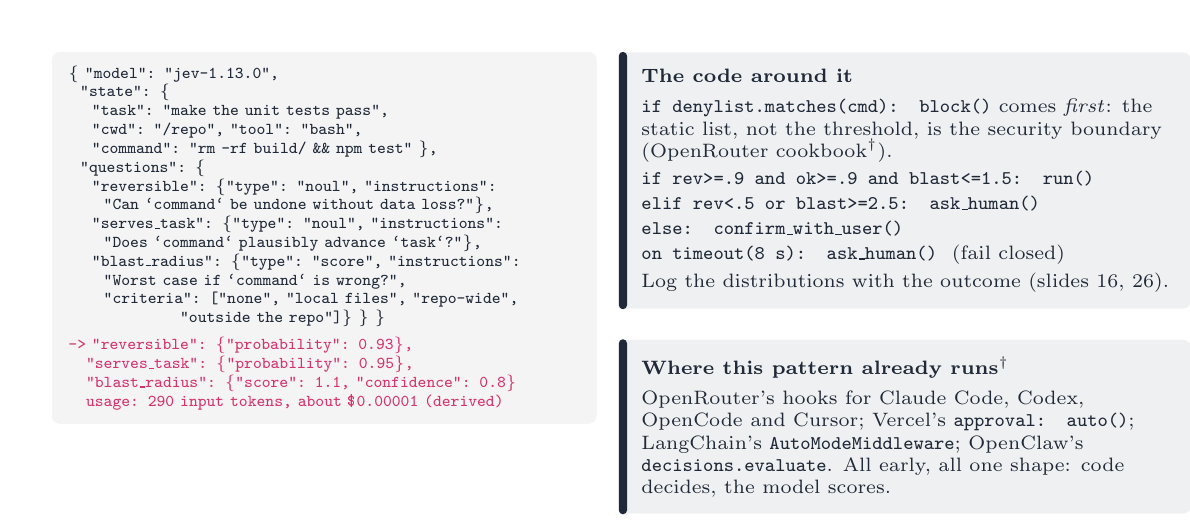
\begin{tikzpicture}
  \useasboundingbox (0,0) rectangle (14.4,5.9);
  \node[anchor=north west,inner sep=0,font=\ttfamily\fontsize{5.8}{6.8}\selectfont,text=ink,
        rounded corners=3pt,fill=ink!5,inner xsep=6pt,inner ysep=5pt,text width=6.5cm,align=left] at (0.3,5.6) {%
    \{ "model": "jev-1.13.0",\\
    \ \ "state": \{\\
    \ \ \ \ "task": "make the unit tests pass",\\
    \ \ \ \ "cwd": "/repo", "tool": "bash",\\
    \ \ \ \ "command": "rm -rf build/ \&\& npm test" \},\\
    \ \ "questions": \{\\
    \ \ \ \ "reversible": \{"type": "noul", "instructions":\\
    \ \ \ \ \ \ "Can `command` be undone without data loss?"\},\\
    \ \ \ \ "serves\_task": \{"type": "noul", "instructions":\\
    \ \ \ \ \ \ "Does `command` plausibly advance `task`?"\},\\
    \ \ \ \ "blast\_radius": \{"type": "score", "instructions":\\
    \ \ \ \ \ \ "Worst case if `command` is wrong?",\\
    \ \ \ \ \ \ "criteria": ["none", "local files", "repo-wide",\\
    \ \ \ \ \ \ \ \ \ \ \ \ \ \ \ \ \ \ \ "outside the repo"]\} \} \}\\[3pt]
    {\color{outc}-> "reversible": \{"probability": 0.93\},}\\
    {\color{outc}\ \ \ "serves\_task": \{"probability": 0.95\},}\\
    {\color{outc}\ \ \ "blast\_radius": \{"score": 1.1, "confidence": 0.8\}}\\
    {\color{outc}\ \ \ usage: 290 input tokens, about \$0.00001 (derived)}};
  \bgpanels{7.5}{5.6}{6.7cm}{The code around it}{%
    \texttt{if denylist.matches(cmd): block()} comes \emph{first}: the
    static list, not the threshold, is the security boundary (OpenRouter
    cookbook$^\dagger$).\\[2pt]
    \texttt{if rev>=.9 and ok>=.9 and blast<=1.5: run()}\\[1pt]
    \texttt{elif rev<.5 or blast>=2.5: ask\_human()}\\[1pt]
    \texttt{else: confirm\_with\_user()}\\[1pt]
    \texttt{on timeout(8 s): ask\_human()} \ (fail closed)\\[2pt]
    Log the distributions with the outcome (slides 16, 26).}
  \bgpanels{7.5}{1.95}{6.7cm}{Where this pattern already runs$^\dagger$}{%
    OpenRouter's hooks for Claude Code, Codex, OpenCode and Cursor;
    Vercel's \texttt{approval: auto()}; LangChain's
    \texttt{AutoModeMiddleware}; OpenClaw's \texttt{decisions.evaluate}.
    All early, all one shape: code decides, the model scores.}
\end{tikzpicture}
\end{frame}

% ---------------------------------------------------------------- 29
\begin{frame}{Writing questions that work}
\framesubtitle{What the docs advise, what the independent tests add, and what to log so you can prove it later.}
\centering
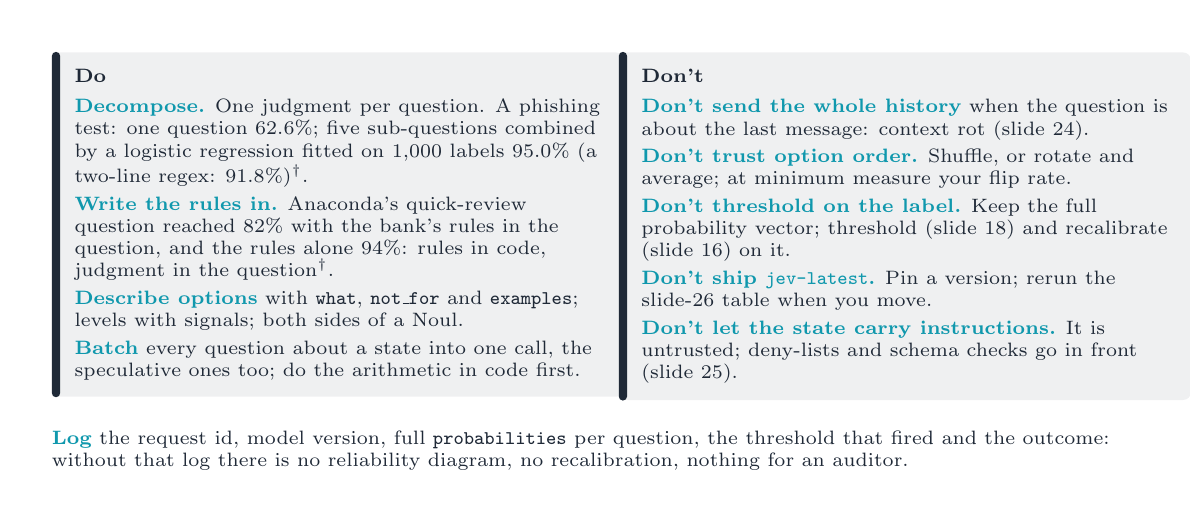
\begin{tikzpicture}
  \useasboundingbox (0,0) rectangle (14.4,5.9);
  \bgpanels{0.3}{5.6}{6.7cm}{Do}{%
    \hl{vc}{Decompose.} One judgment per question. A phishing test: one
    question 62.6\%; five sub-questions combined by a logistic regression
    fitted on 1{,}000 labels 95.0\% (a two-line regex: 91.8\%)$^\dagger$.\\[2pt]
    \hl{vc}{Write the rules in.} Anaconda's quick-review question reached
    82\% with the bank's rules in the question, and the rules alone
    94\%: rules in code, judgment in the question$^\dagger$.\\[2pt]
    \hl{vc}{Describe options} with \texttt{what}, \texttt{not\_for} and
    \texttt{examples}; levels with signals; both sides of a Noul.\\[2pt]
    \hl{vc}{Batch} every question about a state into one call, the
    speculative ones too; do the arithmetic in code first.}
  \bgpanels{7.5}{5.6}{6.7cm}{Don't}{%
    \hl{vc}{Don't send the whole history} when the question is about
    the last message: context rot (slide 24).\\[2pt]
    \hl{vc}{Don't trust option order.} Shuffle, or rotate and average;
    at minimum measure your flip rate.\\[2pt]
    \hl{vc}{Don't threshold on the label.} Keep the full probability
    vector; threshold (slide 18) and recalibrate (slide 16) on it.\\[2pt]
    \hl{vc}{Don't ship \texttt{jev-latest}.} Pin a version; rerun the
    slide-26 table when you move.\\[2pt]
    \hl{vc}{Don't let the state carry instructions.} It is untrusted;
    deny-lists and schema checks go in front (slide 25).}
  \node[txt,anchor=north west,text width=13.8cm,font=\scriptsize] at (0.3,0.78) {%
    \hl{vc}{Log} the request id, model version, full \texttt{probabilities}
    per question, the threshold that fired and the outcome: without that log
    there is no reliability diagram, no recalibration, nothing for an auditor.};
\end{tikzpicture}
\end{frame}

% ---------------------------------------------------------------- 30
\begin{frame}{Build your own: three recipes, in increasing effort}
\framesubtitle{A readout with a temperature, a head on a frozen model, or a fine-tuned encoder; the vendor's number is the floor.}
\centering
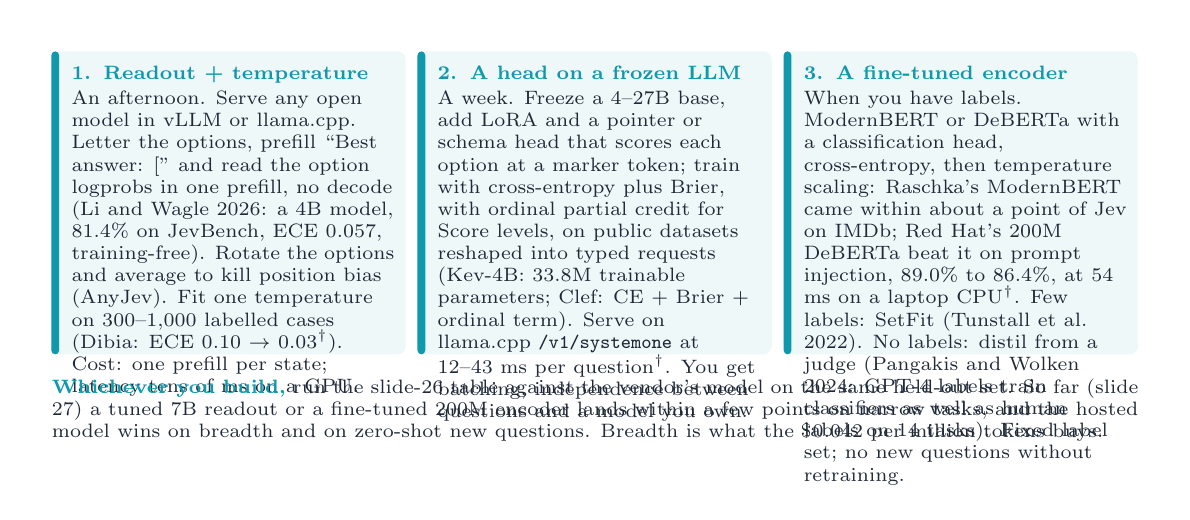
\begin{tikzpicture}
  \useasboundingbox (0,0) rectangle (14.4,5.9);
  \foreach \x/\c/\ttl/\body in {
      0.3/vc/{1. Readout + temperature}/{An afternoon. Serve any open model in vLLM or llama.cpp. Letter the options, prefill ``Best answer: ['' and read the option logprobs in one prefill, no decode (Li and Wagle 2026: a 4B model, 81.4\% on JevBench, ECE 0.057, training-free). Rotate the options and average to kill position bias (AnyJev). Fit one temperature on 300--1{,}000 labelled cases (Dibia: ECE 0.10 $\to$ 0.03$^\dagger$). Cost: one prefill per state; latency tens of ms on a GPU.},
      4.95/vc/{2. A head on a frozen LLM}/{A week. Freeze a 4--27B base, add LoRA and a pointer or schema head that scores each option at a marker token; train with cross-entropy plus Brier, with ordinal partial credit for Score levels, on public datasets reshaped into typed requests (Kev-4B: 33.8M trainable parameters; Clef: CE $+$ Brier $+$ ordinal term). Serve on llama.cpp \texttt{/v1/systemone} at 12--43 ms per question$^\dagger$. You get batching, independence between questions and a model you own.},
      9.6/vc/{3. A fine-tuned encoder}/{When you have labels. ModernBERT or DeBERTa with a classification head, cross-entropy, then temperature scaling: Raschka's ModernBERT came within about a point of Jev on IMDb; Red Hat's 200M DeBERTa beat it on prompt injection, 89.0\% to 86.4\%, at 54 ms on a laptop CPU$^\dagger$. Few labels: SetFit (Tunstall et al.\ 2022). No labels: distil from a judge (Pangakis and Wolken 2024: GPT-4 labels train classifiers as well as human labels on 14 tasks). Fixed label set; no new questions without retraining.}}{
    \fill[\c!7,rounded corners=3pt] (\x,1.75) rectangle (\x+4.5,5.6);
    \fill[\c,rounded corners=1.5pt] (\x,1.75) rectangle (\x+0.1,5.6);
    \node[anchor=north west,font=\scriptsize\bfseries,text=\c,inner sep=0,text width=4.1cm] at (\x+0.25,5.42) {\ttl};
    \node[anchor=north west,font=\fontsize{6.6}{8}\selectfont,text=ink,inner sep=0,text width=4.1cm,align=flush left] at (\x+0.25,5.1) {\body};}
  \node[txt,anchor=north west,text width=13.8cm,font=\scriptsize] at (0.3,1.45) {%
    \hl{vc}{Whichever you build,} run the slide-26 table against the
    vendor's model on the same held-out set. So far (slide 27) a tuned 7B
    readout or a fine-tuned 200M encoder lands within a few points on
    narrow tasks, and the hosted model wins on breadth and on zero-shot
    new questions. Breadth is what the \$0.042 per million tokens buys.};
\end{tikzpicture}
\end{frame}

% ---------------------------------------------------------------- 31
\stage{10}
\begin{frame}{Summary: what to take from this lecture}
\framesubtitle{Calibrated classification as a service: the science is old, the economics are new, the evidence is young.}
\centering
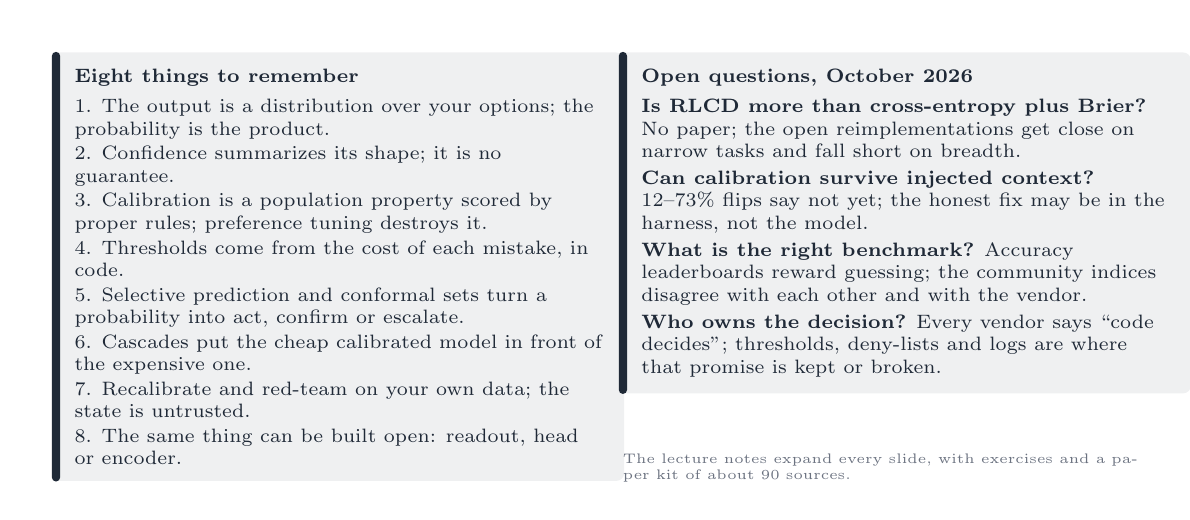
\begin{tikzpicture}
  \useasboundingbox (0,0) rectangle (14.4,5.9);
  \bgpanels{0.3}{5.6}{6.7cm}{Eight things to remember}{%
    1. The output is a distribution over your options; the probability
    is the product.\\[1pt]
    2. Confidence summarizes its shape; it is no guarantee.\\[1pt]
    3. Calibration is a population property scored by proper rules;
    preference tuning destroys it.\\[1pt]
    4. Thresholds come from the cost of each mistake, in code.\\[1pt]
    5. Selective prediction and conformal sets turn a probability into
    act, confirm or escalate.\\[1pt]
    6. Cascades put the cheap calibrated model in front of the
    expensive one.\\[1pt]
    7. Recalibrate and red-team on your own data; the state is
    untrusted.\\[1pt]
    8. The same thing can be built open: readout, head or encoder.}
  \bgpanels{7.5}{5.6}{6.7cm}{Open questions, October 2026}{%
    \hl{ink}{Is RLCD more than cross-entropy plus Brier?} No paper; the
    open reimplementations get close on narrow tasks and fall short on
    breadth.\\[2pt]
    \hl{ink}{Can calibration survive injected context?} 12--73\% flips
    say not yet; the honest fix may be in the harness, not the
    model.\\[2pt]
    \hl{ink}{What is the right benchmark?} Accuracy leaderboards reward
    guessing; the community indices disagree with each other and with
    the vendor.\\[2pt]
    \hl{ink}{Who owns the decision?} Every vendor says ``code decides'';
    thresholds, deny-lists and logs are where that promise is kept or
    broken.}
  \node[lab,anchor=north west,text width=6.7cm,font=\tiny] at (7.5,0.55) {The lecture notes expand every slide, with exercises and a paper kit of about 90 sources.};
\end{tikzpicture}
\end{frame}

% ---------------------------------------------------------------- 32
\begin{frame}{Sources}
\framesubtitle{Documentation and model cards, papers, and the independent tests quoted; $^\dagger$ marks vendor and community material.}
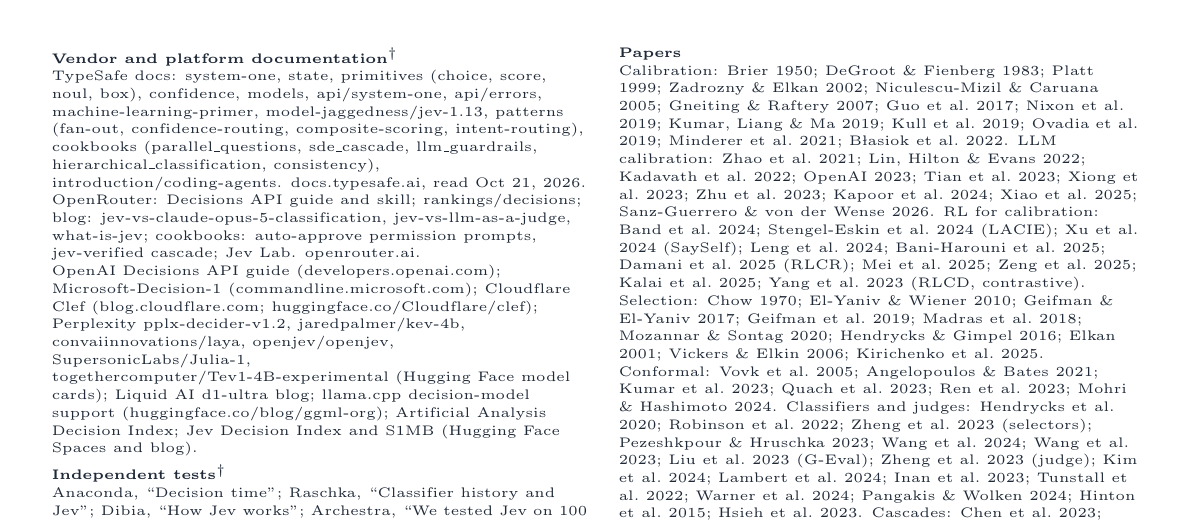
\begin{tikzpicture}
  \useasboundingbox (0,0) rectangle (14.4,5.9);
  \node[anchor=north west,inner sep=0,text width=6.8cm,font=\fontsize{5.4}{6.4}\selectfont,text=ink,align=flush left] at (0.3,5.65) {%
    \textbf{Vendor and platform documentation$^\dagger$}\\
    TypeSafe docs: system-one, state, primitives (choice, score, noul, box), confidence, models, api/system-one, api/errors, machine-learning-primer, model-jaggedness/jev-1.13, patterns (fan-out, confidence-routing, composite-scoring, intent-routing), cookbooks (parallel\_questions, sde\_cascade, llm\_guardrails, hierarchical\_classification, consistency), introduction/coding-agents. docs.typesafe.ai, read Oct 21, 2026.\\
    OpenRouter: Decisions API guide and skill; rankings/decisions; blog: jev-vs-claude-opus-5-classification, jev-vs-llm-as-a-judge, what-is-jev; cookbooks: auto-approve permission prompts, jev-verified cascade; Jev Lab. openrouter.ai.\\
    OpenAI Decisions API guide (developers.openai.com); Microsoft-Decision-1 (commandline.microsoft.com); Cloudflare Clef (blog.cloudflare.com; huggingface.co/Cloudflare/clef); Perplexity pplx-decider-v1.2, jaredpalmer/kev-4b, convaiinnovations/laya, openjev/openjev, SupersonicLabs/Julia-1, togethercomputer/Tev1-4B-experimental (Hugging Face model cards); Liquid AI d1-ultra blog; llama.cpp decision-model support (huggingface.co/blog/ggml-org); Artificial Analysis Decision Index; Jev Decision Index and S1MB (Hugging Face Spaces and blog).\\[2pt]
    \textbf{Independent tests$^\dagger$}\\
    Anaconda, ``Decision time''; Raschka, ``Classifier history and Jev''; Dibia, ``How Jev works''; Archestra, ``We tested Jev on 100 real agent calls''; AbdelStark jev-benchmarks; RINNECODER jev-behavior-study; alexmolas, ``Jev can't be calibrated''; Latent Space interview with D.\ Almeida; TechCrunch (Sept 18, Oct 9), Forbes (Sept 15), Business Wire release (Sept 15).};
  \node[anchor=north west,inner sep=0,text width=6.6cm,font=\fontsize{5.4}{6.4}\selectfont,text=ink,align=flush left] at (7.5,5.65) {%
    \textbf{Papers}\\
    Calibration: Brier 1950; DeGroot \& Fienberg 1983; Platt 1999; Zadrozny \& Elkan 2002; Niculescu-Mizil \& Caruana 2005; Gneiting \& Raftery 2007; Guo et al.\ 2017; Nixon et al.\ 2019; Kumar, Liang \& Ma 2019; Kull et al.\ 2019; Ovadia et al.\ 2019; Minderer et al.\ 2021; B\l{}asiok et al.\ 2022. LLM calibration: Zhao et al.\ 2021; Lin, Hilton \& Evans 2022; Kadavath et al.\ 2022; OpenAI 2023; Tian et al.\ 2023; Xiong et al.\ 2023; Zhu et al.\ 2023; Kapoor et al.\ 2024; Xiao et al.\ 2025; Sanz-Guerrero \& von der Wense 2026. RL for calibration: Band et al.\ 2024; Stengel-Eskin et al.\ 2024 (LACIE); Xu et al.\ 2024 (SaySelf); Leng et al.\ 2024; Bani-Harouni et al.\ 2025; Damani et al.\ 2025 (RLCR); Mei et al.\ 2025; Zeng et al.\ 2025; Kalai et al.\ 2025; Yang et al.\ 2023 (RLCD, contrastive). Selection: Chow 1970; El-Yaniv \& Wiener 2010; Geifman \& El-Yaniv 2017; Geifman et al.\ 2019; Madras et al.\ 2018; Mozannar \& Sontag 2020; Hendrycks \& Gimpel 2016; Elkan 2001; Vickers \& Elkin 2006; Kirichenko et al.\ 2025. Conformal: Vovk et al.\ 2005; Angelopoulos \& Bates 2021; Kumar et al.\ 2023; Quach et al.\ 2023; Ren et al.\ 2023; Mohri \& Hashimoto 2024. Classifiers and judges: Hendrycks et al.\ 2020; Robinson et al.\ 2022; Zheng et al.\ 2023 (selectors); Pezeshkpour \& Hruschka 2023; Wang et al.\ 2024; Wang et al.\ 2023; Liu et al.\ 2023 (G-Eval); Zheng et al.\ 2023 (judge); Kim et al.\ 2024; Lambert et al.\ 2024; Inan et al.\ 2023; Tunstall et al.\ 2022; Warner et al.\ 2024; Pangakis \& Wolken 2024; Hinton et al.\ 2015; Hsieh et al.\ 2023. Cascades: Chen et al.\ 2023; Jitkrittum et al.\ 2023; Yue et al.\ 2023; Ong et al.\ 2024; Cheng et al.\ 2023. System 1/2: Kahneman 2011; Booch et al.\ 2020; Yu et al.\ 2024. Decision models: Rafe \& Das 2026; Guo et al.\ 2026; Hu et al.\ 2026; Xu et al.\ 2026; Wu \& Lim 2026; Li \& Wagle 2026; Sharma et al.\ 2026 (TypedBench). Full list with arXiv identifiers in the paper kit.};
\end{tikzpicture}
\end{frame}
\end{document}
